% !TEX root = ../main.tex
This appendix contains the proofs that are not in \Cref{ch:basecases}, and the lemmas they need.
The definitions are in \Cref{ch:basecases}. New terms are defined where they are first used.

The appendix has three parts.
\textsc{Part I} is about undirected graphs, \textsc{Part II} about directed graphs, and \textsc{Part III} about hypergraphs.
The three main proof ideas are the reachability skeleton (directed multigraphs), the incidence-rank lemma (hypergraphs at $m=3$), and the two-step budget (directed graphs and hypergraphs).



% ---------------------------------------------------------------------------
% Part dividers. The appendix is one chapter, so its thirteen sections would
% otherwise present as a flat list longer than any body chapter. \apppart draws
% a labelled rule before each group and writes the group into the table of
% contents, so a reader can find the directed work or the hypergraph work
% without scanning every section heading. It introduces no numbering and no new
% label, so every \Cref{app:proofs} in the body still resolves to this chapter.
% ---------------------------------------------------------------------------
\newcommand{\apppart}[2]{%
  \par\addvspace{1.2\baselineskip}%
  \Needspace{8\baselineskip}%
  \phantomsection% own anchor, so the bookmark does not collide with the chapter's
  \addcontentsline{toc}{section}{\protect\numberline{}\textsc{#1}}%
  \noindent{\color{KULblauw1}\rule{\linewidth}{1.1pt}}\par\nobreak
  \vspace{2pt}\noindent{\normalfont\bfseries\color{KULblauw1}#1}\par\nobreak
  \vspace{1pt}\noindent{\normalfont\small\itshape\color{black!70}#2}\par\nobreak
  \vspace{2pt}\noindent{\color{KULblauw1}\rule{\linewidth}{0.4pt}}\par\nobreak
  \addvspace{0.4\baselineskip}}

\clearpage
\apppart{Part I. Undirected graphs}{Graphs that attain Mader's bound, and the vertex problem as a problem about blocks.}

\section{Graphs that attain Mader's bound}\label{sec:mader-extremal}

The constructions below need hypergraphs in which no vertex lies in too many hyperedges. Recall that a graph is a $2$-uniform hypergraph, and the \emph{degree} of a vertex is the number of hyperedges that contain it.

\begin{lemma}[Sparse uniform hypergraphs exist]\label{lem:sparse-hypergraph}
Let $r$, $n$ and $d$ be integers with $r \ge 1$, $n \ge r$ and $0 \le d \le \binom{n-1}{r-1}$. There is a simple
$r$-uniform hypergraph on $n$ vertices with exactly $\floorfrac{dn}{r}$
hyperedges and maximum degree at most $d$.
\end{lemma}

\begin{proof}
Let $N := \floorfrac{dn}{r}$. Then $N \le \frac{n}{r}\binom{n-1}{r-1} = \binom{n}{r}$, so there are at least $N$ different $r$-sets.
Among all families of $N$ different $r$-sets, choose one with the smallest value of $\sum_x \deg(x)^2$.
Suppose $\deg(x) \ge \deg(y) + 2$ for two vertices $x,y$.
Let $a$ be the number of sets in the family that contain $x$ but not $y$, and $b$ the number that contain $y$ but not $x$. Then $a \ge b + 2$.
The map $A \mapsto A - x + y$ sends the first kind of set to the second kind, and different sets have different images.
Since $a>b$, some image $A - x + y$ is not in the family.
Replace $A$ by $A - x + y$. The family stays simple and has $N$ sets, and the sum changes by
\[
(\deg(x)-1)^2 + (\deg(y)+1)^2 - \deg(x)^2 - \deg(y)^2
 = 2\bigl(\deg(y) - \deg(x)\bigr) + 2 \le -2.
\]
This contradicts the choice of the family.
So any two degrees differ by at most one.
The degrees add up to $rN \le dn$, so the largest degree is $\ceil{rN/n} \le d$.
\end{proof}


\begin{construction}[Hub-and-spokes graph]\label{const:hub-spokes}\label{const:shared-clique}
Let $n\ge m\ge2$. The graph $H_{m,n}$ has a vertex $h$ and further vertices $v_1,\dots,v_{n-1}$. Join $h$ to every $v_i$. On $v_1,\dots,v_{n-1}$, add a graph with $\floor{(m-2)(n-1)/2}$ edges in which every vertex has degree at most $m-2$. For $n\ge3$ such a graph exists by \Cref{lem:sparse-hypergraph} with uniformity $2$. If $m-1$ divides $n-1$, one can take disjoint copies of $K_{m-1}$. Then $H_{m,n}$ consists of copies of $K_m$ that share the vertex $h$.
\end{construction}





\begin{theorem}[Extremal graphs exist]\label{thm:extremal-existence}
For all $n \ge m \ge 2$ the graph $H_{m,n}$ has $\floorfrac{m(n-1)}{2}$ edges and $\lec^{\max} \le m-1$.
\end{theorem}

\begin{proof}
The number of edges is $(n-1) + \floorfrac{(m-2)(n-1)}{2} = \floorfrac{m(n-1)}{2}$.
Of any two vertices, at least one is some $v_i$.
This vertex has degree at most $1 + (m-2) = m-1$.
So \Cref{lem:degree-bound} gives $\lec(u,v) \le m-1$.
\end{proof}

So for $n\ge m$ the bound of \Cref{thm:mader} is attained.
The next theorem describes what equality means for the Gomory--Hu tree.

\begin{theorem}[Equality in the Gomory--Hu bound]\label{thm:extremal-char}
Let $G$ be simple with $\lec^{\max}_G \le m-1$ and $|E(G)| = \floorfrac{m(n-1)}{2}$, and let $T$ be a Gomory--Hu tree of $G$.
\begin{enumerate}[label=(\alph*)]
\item If $m(n-1)$ is even, then every tree edge has weight $m-1$, every tree edge is an edge of $G$, and every edge of $G$ has $\dist_T(e)\le2$.
\item If $m(n-1)$ is odd, then exactly one of these three statements fails, and it fails by one: one tree edge has weight $m-2$, or one tree edge is not an edge of $G$, or one edge of $G$ has $\dist_T(e)=3$.
\end{enumerate}
\end{theorem}

\begin{proof}
Each inequality in the proof of \Cref{thm:mader} has a non-negative integer gap:
\[
    S_1 = (m-1)(n-1) - \sum_t c(t),
    \qquad
    S_2 = \sum_{e :\, \dist_T(e) \ge 2} \bigl(\dist_T(e) - 2\bigr),
    \qquad
    S_3 = (n-1) - |E_1| .
\]
Here $S_1$ counts tree weights below $m-1$, $S_2$ counts how far edges go beyond tree distance two, and $S_3$ counts tree edges that are not edges of $G$.
The proof gives two expressions for the same sum:
\[
    \sum_e \dist_T(e) \;=\; 2|E| - |E_1| + S_2
    \qquad\text{and}\qquad
    \sum_e \dist_T(e) \;=\; \sum_t c(t) \;=\; (m-1)(n-1) - S_1 .
\]
We substitute $|E_1| = (n-1) - S_3$ into the first and compare with the second:
\[
\begin{aligned}
    2|E| - (n-1) + S_2 + S_3 &\;=\; (m-1)(n-1) - S_1, \\[2pt]
    \text{so}\qquad 2|E| &\;=\; m(n-1) - (S_1 + S_2 + S_3).
\end{aligned}
\]
If $m(n-1)$ is even, then $|E| = m(n-1)/2$ forces $S_1 = S_2 = S_3 = 0$.
If $m(n-1)$ is odd, then $|E| = (m(n-1)-1)/2$ gives $S_1 + S_2 + S_3 = 1$, so exactly one gap equals one.
\end{proof}

For $m = 2$ this shows that the extremal graphs are exactly the trees on the $n$ vertices.
Indeed, every tree edge then has weight one and is an edge of $G$, so $G$ contains $T$ and has only $n-1$ edges.

\begin{remark}[Forcing and avoiding counts]\label{rem:threshold-convention}\label{rem:threshold-audit}
This thesis maximises the number of edges with no $m$ disjoint routes between any pair.
S{\o}rensen and Thomassen, and the Erd\H{o}s Problems database, give instead the least number of edges that forces such a pair \cite{SorensenThomassen74,ErdosProblems}.
Their number is one more than ours.

For example, Theorem~4 of \cite{SorensenThomassen74} gives the forcing number $\floor{8n/3}-3$ for $n\ge6$, except $16$ at $n=7$ and $28$ at $n=12$.
Subtracting one gives our values.
For $6\le n\le13$ these numbers, the two exceptions included, equal $\floor{5(n-1)/2}+1$.
Subtracting one gives the two cases of \Cref{thm:sorensen-thomassen}.
At $n=13$ both maxima are $30$, and the edge and vertex values first differ at $n=14$.

The same care is needed for the Bollob\'{a}s--Erd\H{o}s conjecture of \Cref{sec:simple-vertex-blocks}.
Its forcing number $1+\binom m2 p$ is for graphs on $1+(m-1)p$ vertices.
Each copy of $K_m$ adds $\binom m2$ edges but only $m-1$ vertices, so in our notation the rate is $m/2$ edges per vertex.
\end{remark}

\subsection{The vertex problem is a block problem}\label{sec:simple-vertex-blocks}

The vertex problem $k_m(n)$ is open for $m\ge6$.
This section reduces it to $2$-connected graphs (\Cref{thm:simple-vertex-blocks}).

A graph on more than $k$ vertices is \emph{$k$-connected} if removing any $k-1$ vertices leaves it connected.
A \emph{cut vertex} is a vertex whose removal disconnects the graph.
A \emph{bridge} is an edge whose removal disconnects its component.
A \emph{block} is a maximal connected subgraph that has an edge and no cut vertex of its own.
In a simple graph, a block is either a bridge or a maximal $2$-connected subgraph.

The next theorem says that the best graph is built from blocks: choose block sizes $b_i$, where a block of size $b_i$ costs $b_i-1$ vertices and gives at most $h_m(b_i)$ edges, with total cost at most $n-1$.

\begin{theorem}[The vertex problem reduces to blocks]\label{thm:simple-vertex-blocks}
For $b \ge 2$ let
\[
    h_m(b) \;:=\; \max\bigl\{\, |E(B)| \;:\; B \text{ $2$-connected or a single edge},\ |V(B)| = b,\ \kap^{\max}_B \le m-1 \,\bigr\} ,
\]
with $h_m(b) := -\infty$ when no such $B$ exists.
Then for all $m \ge 2$ and $n \ge 2$,
\[
    k_m(n) \;=\; \max\Bigl\{\, \sum_i h_m(b_i) \;:\; b_i \ge 2,\ \sum_i (b_i - 1) \le n-1 \,\Bigr\} .
\]
Consequently $k_m(n) \ge k_m(n_1) + k_m(n_2)$ whenever $n = n_1 + n_2 - 1$, and
\[
    c_m \;:=\; \lim_{n \to \infty} \frac{k_m(n)}{n-1} \;=\; \sup_{b \ge 2} \frac{h_m(b)}{b-1}
\]
exists, the limit being approached from below. The supremum is finite: \Cref{rem:vertex-degeneracy} gives $k_m(n) < 2(m-1)n$, so $c_m \le 2(m-1)$.
\end{theorem}

\begin{proof}
Let $G$ be feasible, and let $u,v$ lie in a common block $B$.
No $u$--$v$ path leaves $B$: it would have to leave and come back through the same cut vertex, and a path visits each vertex once.
So $\kap_G(u,v) = \kap_B(u,v)$.
Every block is a subgraph of $G$, so it is feasible too.
Every edge lies in exactly one block, so $|E(G)| = \sum_B |E(B)| \le \sum_B h_m(|V(B)|)$.
In each component, $\sum_B (|V(B)|-1)$ is the number of vertices minus one.
So over all of $G$, $\sum_B (|V(B)|-1) \le n-1$.
This proves $\le$.

For $\ge$, take blocks $B_1, \dots, B_t$ with $\sum (b_i - 1) \le n-1$.
Glue them at one common vertex, and keep them disjoint otherwise.
This graph has $1 + \sum(b_i-1) \le n$ vertices. Add isolated vertices to reach $n$.
Its blocks are the $B_i$, so pairs inside one block keep their value of $\kap$.
Two vertices in different blocks are separated by the common vertex, so $\kap \le 1 \le m-1$.
So the graph is feasible, with $\sum_i |E(B_i)|$ edges.

Gluing two extremal graphs at one vertex gives $k_m(n) \ge k_m(n_1) + k_m(n_2)$ for $n = n_1 + n_2 - 1$.

For the limit, write $a_n = k_m(n)/(n-1)$ and $s = \sup_{b \ge 2} h_m(b)/(b-1)$.
By the display, $k_m(n) \le s\,(n-1)$, so $a_n \le s$ for every $n$.
Fekete's lemma \cite{Fekete23} says: if numbers $x_1, x_2, \dots$ satisfy $x_{i+j} \ge x_i + x_j$, then $x_t/t$ tends to $\sup_t x_t/t$.
We apply it to $x_t = k_m(t+1)$, which satisfies this by the gluing inequality.
So $a_n$ tends to $\sup_n a_n$.
This supremum is $s$: it is at most $s$, and $a_b \ge h_m(b)/(b-1)$ for every $b$, since one block of size $b$ is a graph on $b$ vertices.
\end{proof}

We note three consequences.

First, at $m = 3$ the reduction gives \Cref{thm:leonard} again.
A block with $\kap^{\max} \le 2$ is an edge or a cycle.
Otherwise it contains a \emph{theta}: three internally disjoint paths with the same two ends, which break the condition.
So $h_3(2) = 1$ and $h_3(b) = b$ for $b \ge 3$.
The rate $b/(b-1)$ is largest at $b = 3$, so the best choice uses triangles:
$k_3(n) = 3\floor{(n-1)/2} + ((n-1) \bmod 2) = \floorfrac{3(n-1)}{2}$.

Second, at $m = 4$, \Cref{thm:leonard} gives $h_4(b) = 2(b-1)$ for every $b \ge 4$.
So the rate $h_4(b)/(b-1)$ is $2$ for $b\ge4$, against $1$ at $b = 2$ and $3/2$ at $b = 3$.
The best choice uses blocks of size at least four, and $k_4(n) = 2(n-1)$ for $n \ge 4$.
This uses \Cref{thm:leonard}, so it is not a new proof.
It does show the extremal block: the hub-and-spokes graph $H_{4,b}$ of \Cref{const:hub-spokes}, which is a hub joined to all vertices of a cycle.
It is a single block with $2(b-1)$ edges.

Third, the Bollob\'as--Erd\H{o}s construction, copies of $K_m$ sharing one vertex, is the case $b = m$: $h_m(m) = \binom{m}{2}$, with rate $m/2$.
Their conjecture says that $c_m = m/2$, so that no block beats $K_m$.
A \emph{bouquet} is a set of blocks that share one vertex and are otherwise disjoint.
Its rate is a weighted average of the rates of its blocks.
So a counterexample must contain one $2$-connected block with rate above $m/2$.

The conjecture is false. S\o{}rensen and Thomassen \cite{SorensenThomassen74} showed that for each fixed $m$,
\[
    c_m \;\ge\; \frac{m(m-1)-2}{2m-3} \;=\; \frac{m}{2} + \frac{1}{4} + O(1/m).
\]
This is larger than $m/2$ for every $m \ge 5$, because
\[
    2\bigl(m(m-1)-2\bigr) - m(2m-3) \;=\; m-4 .
\]

Their example is built step by step.
Start with $G^0 = K_m$ minus an edge.
To build $G^{j}$, take $G^{j-1}$ and two new copies of $G^0$, and glue them in a cycle: each one shares one vertex with the next.
Each step adds $2m-3$ vertices and $m(m-1)-2$ edges, which gives the rate above.
Gluing in a cycle creates no cut vertex, so $G^{j}$ is a single block.
So \Cref{thm:simple-vertex-blocks} sees $G^j$ as one block of size $m + (2m-3)j$ and does not help to find it.
The recursion beats the rate $m/2$ only when $j > 2/(m-4)$.
So the smallest member of this family that beats copies of $K_m$ has $26$ vertices at $m = 5$, $24$ at $m = 6$ and $18$ at $m = 7$.
Smaller examples exist. At $m=5$, \Cref{thm:sorensen-thomassen} gives $33$ edges on $14$ vertices, and by the bouquet argument above such a graph contains a block with rate above $5/2$.
So $c_m=m/2$ for $m\le4$, $c_5=8/3$ by \Cref{thm:sorensen-thomassen}, and $m/2<c_m\le2(m-1)$ for $m\ge6$.

\begin{remark}[A question about small degrees]\label{rem:vertex-degeneracy}
Mader's density theorem \cite{Mader72}, in the form of \cite[Theorem~1.4.3]{Diestel17}, says that a graph of average degree at least $4k$ has a $(k+1)$-connected subgraph. A graph with at least $2(m-1)n$ edges has average degree at least $4(m-1)$, so it has an $m$-connected subgraph, and two of its vertices are joined by $m$ internally disjoint paths. So $k_m(n) < 2(m-1)n$.
Feasibility gives more. For example, two adjacent vertices have at most $m-2$ common neighbours, since each common neighbour gives a route of length two next to the edge.

We ask whether every feasible graph has a vertex of degree at most $m-1$.
Feasibility passes to induced subgraphs.
So a positive answer would mean that every non-empty induced subgraph has a vertex of degree at most $m-1$.
Removing such vertices one by one would give
\[
    k_m(n) \;\le\; \sum_{i=1}^{n}\min(i-1,\,m-1) \;=\; (m-1)n - \binom{m}{2}
    \qquad (n \ge m-1),
\]
half the constant of Mader's bound.

The answer is yes for $m = 3$.
By a theorem of Dirac \cite{Dirac52}, a graph of minimum degree at least three contains a \emph{subdivision} of $K_4$: a copy of $K_4$ in which edges are replaced by internally disjoint paths.
Two of its four main vertices are joined by three internally disjoint paths, which breaks the condition at $m=3$.
For $m\ge4$ the question is open.
\end{remark}

\apppart{Part II. Directed graphs}{The directed constructions, the reachability skeleton, the bounds for $m\ge3$, and the extremal directed multigraphs.}

\section{The directed constructions}\label{sec:dir-constructions}

Three constructions give the directed lower bounds.
\Cref{fig:simple-digraph-m2} shows the first two.
Here we define them and check their connectivity.

\begin{construction}[Directed hub]\label{const:directed-hub}
For $n \ge m \ge 2$, take a hub $h$ and label the other $N = n-1$ vertices $0, \dots, N-1$. Add the $2N$ hub arcs $h \to i$ and $i \to h$, and on the non-hub vertices the $(m-2)N$ ring arcs $i \to i+j \bmod N$ for $j = 1, \dots, m-2$. The total is $m(n-1)$ arcs and every non-hub vertex has $d^+ = d^- = m-1$.
\end{construction}

Every ordered pair contains a vertex other than the hub, and that vertex has out-degree and in-degree $m-1$.
So the degree bound gives $\lec^{\max} \le m-1$.
At $m = 2$ there are no ring arcs, and we get the \emph{bidirected star}.

\begin{construction}[One-directional bipartite digraph]\label{const:bipartite}
Split the vertices into parts $A$ and $B$ of sizes $\floor{n/2}$ and $\ceil{n/2}$, and include every arc from $A$ to $B$ and none the other way. The total is $\floor{n^2/4}$ arcs.
\end{construction}

No arc leaves $B$ and no arc enters $A$.
So every route has length one, and $\lec^{\max} = 1$.

\begin{construction}[Augmented bipartite digraph]\label{const:augmented-bipartite}
For $n \ge m \ge 2$, set $|B| = \ceil{(n+m-2)/2}$ and $|A| = n - |B|$, include every arc from $A$ to $B$, and inside $B$ give each $b_j$ the $m-2$ in-arcs from its cyclic predecessors $b_{j-1}, \dots, b_{j-(m-2)}$. The total is $\floor{(n+m-2)^2/4}$ arcs.
\end{construction}

\Cref{lem:augmented-feasible} shows that $\lec^{\max}=m-1$.
For example, take $m = 3$ and $n = 10$.
Then $|B| = 6$ and $|A| = 4$.
There are $24$ arcs from $A$ to $B$, and $6$ arcs forming a cycle inside $B$.
Each pair $a_i, b_j$ has the direct arc and one detour, so $\lec^{\max} = 2$.
This gives $30$ arcs, more than the $\max(m(n-1),\floor{n^2/4})=27$ of the first two constructions.
The gain comes from making $B$ larger than half of the vertices.
So for $n\ge m$,
\[
    \ell_m^{\mathrm{dir}}(n)\;\ge\;\max\Bigl(m(n-1),\ \floorfrac{(n+m-2)^2}{4}\Bigr).
\]
For fixed $m$ and large $n$ the augmented bipartite digraph has more arcs (\Cref{fig:crossover,fig:augmented-wall}).

\begin{figure}[t]
    \centering
    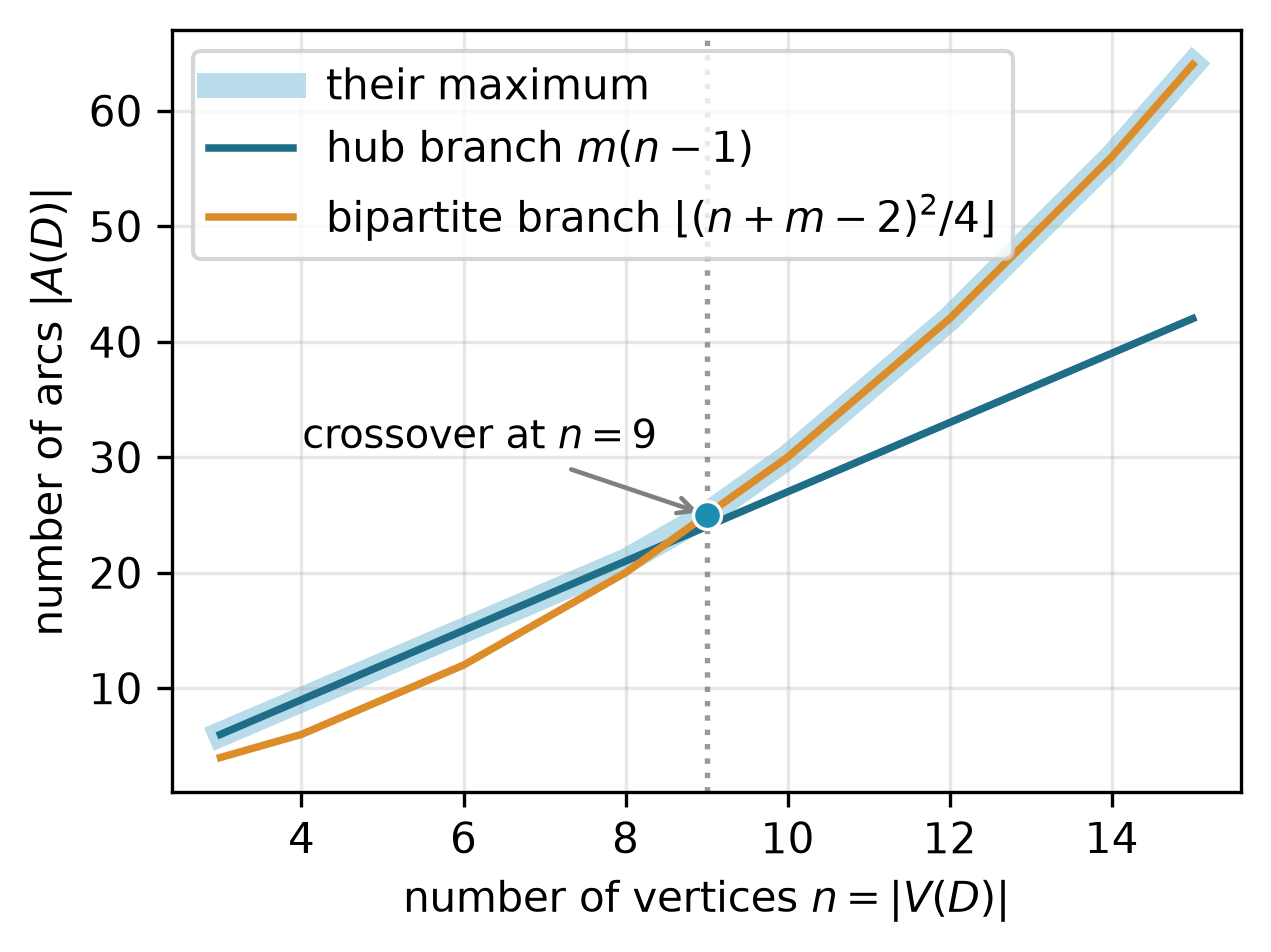
\includegraphics[width=0.78\textwidth]{figures/directed_crossover.png}
    \caption{The arc counts of the hub and of the augmented bipartite digraph at $m = 3$, and their maximum. These are lower bounds only.}
    \label{fig:crossover}
\end{figure}

\begin{figure}[t]
\centering
\begin{tikzpicture}[>=Stealth, scale=1.0,
    wallarc/.style={gdirfaint},
    cyc/.style={-{Stealth[length=2.4mm]}, line width=1.3pt, vertexorange!85!black}]

  % The m = 3, n = 10 instance: |A| = 4, |B| = 6. B is drawn as the ring its
  % m-2 = 1 cyclic in-arc per vertex actually forms, rather than as a second
  % column, where six arcs along one side merge into a single visible stroke.
  \foreach \i/\y in {1/1.65, 2/0.55, 3/-0.55, 4/-1.65} {
    \node[smallvertex] (a\i) at (0,\y) {$a_{\i}$};
  }
  \foreach \j/\ang in {1/90, 2/30, 3/-30, 4/-90, 5/-150, 6/150} {
    \node[smallvertex] (b\j) at ($(5.6,0)+(\ang:1.85)$) {$b_{\j}$};
  }
  \begin{scope}[on background layer]
    \node[draw=KULblauw1!25, fill=KULblauw1!6, rounded corners=10pt,
          fit={(a1) (a4)}, inner sep=9pt] {};
    \node[draw=vertexorange!35, fill=vertexorange!5, circle,
          fit={(b1) (b2) (b3) (b4) (b5) (b6)}, inner sep=1pt] {};
  \end{scope}
  \node[font=\scriptsize, KULblauw1] at (0,2.55) {part $A$};
  \node[font=\scriptsize, vertexorange!75!black] at (5.6,2.55) {part $B$};

  % every arc from A to B: 4 x 6 = 24
  \foreach \i in {1,...,4}{\foreach \j in {1,...,6}{\draw[wallarc] (a\i) -- (b\j);}}

  % inside B, each b_j takes its m-2 = 1 cyclic predecessor: 6 more arcs
  \foreach \j/\k in {1/2, 2/3, 3/4, 4/5, 5/6, 6/1} {
    \draw[cyc] (b\j) -- (b\k);
  }

  \node[font=\scriptsize] at (0,-2.55) {$24$ arcs $A \to B$};
  \node[font=\scriptsize, align=center, vertexorange!75!black] at (5.6,-2.55)
    {$6$ cyclic in-arcs inside $B$};
\end{tikzpicture}
\caption{The augmented bipartite digraph of \Cref{const:augmented-bipartite} at $m = 3$, $n = 10$. All arcs between the parts go from $A$ to $B$. Inside $B$, each vertex gets one arc from the previous vertex on a cycle. A pair $a_i, b_j$ has the direct arc and one detour, so $\lec^{\max} = 2$. The digraph has $24 + 6 = 30$ arcs, against $27$ for the hub.}
\label{fig:augmented-wall}
\end{figure}


\section{The reachability skeleton}\label{sec:reach-skeleton}

The next lemma is used for both exact directed results.
The proofs of \Cref{thm:dir-vertex-m2-exact,thm:dir-multi-full} in \Cref{ch:basecases} use it.

\begin{definition}[Reachability skeleton]\label{def:reach-skeleton}
Let $D$ be a directed multigraph. A \emph{reachability skeleton} of $D$ is a subdigraph $R$ on the same vertices, with at most one copy of each arc, such that for all $u\ne v$: $u$ can reach $v$ in $R$ exactly when $u$ can reach $v$ in $D$.
\end{definition}

A skeleton keeps the information about who can reach whom. It does not keep the number of disjoint paths.

\begin{lemma}[A sparse reachability skeleton always exists]\label{lem:reach-skeleton}
Every loopless directed multigraph $D$ on $n \ge 2$ vertices has a reachability skeleton $R$ with $|A(R)| \le M(n)$.
\end{lemma}

\begin{proof}
We build $R$ in three steps: first inside each strongly connected component, then between components, and then we count.
A \emph{strongly connected component} is a maximal set of vertices in which any two can reach each other.
Every digraph splits into such components.
\Cref{fig:skeleton-example} shows an example.

\emph{Step 1: inside each component.}
Take a component with $n_i$ vertices and choose a vertex $r$ in it.
Since $r$ can reach every vertex of the component, there is an \emph{out-tree}: $n_i-1$ arcs, all pointing away from $r$, along which $r$ reaches every vertex.
(Grow it one arc at a time.)
In the same way there is an \emph{in-tree} of $n_i-1$ arcs, along which every vertex reaches $r$.
Any two vertices $u,v$ of the component are then joined by a walk $u\to r\to v$ in these two trees, which contains a path.
So at most $2(n_i - 1)$ arcs keep all reachability inside the component.

\emph{Step 2: between components.}
Replace each component by one point.
Put an arc from one point to another if $D$ has an arc from the first component to the second.
This gives a digraph $Q_0$ on $q$ points, one per component.
$Q_0$ has no directed cycle, since a cycle would merge components.
Now delete arcs from $Q_0$ one at a time, as long as this does not change who can reach whom.
Call the result $Q$.

The graph $Q$, with directions ignored, has no triangle.
Indeed, suppose three points $x, y, z$ of $Q$ are joined in pairs.
Since $Q$ has no directed cycle, the three arcs must look like $x \to y$, $y \to z$ and $x \to z$, after renaming.
But then $x \to z$ could be deleted, since $x$ still reaches $z$ through $y$.
This contradicts the choice of $Q$.
By Mantel's theorem \cite{Mantel07,Turan41}, a triangle-free graph on $q$ vertices has at most $\floor{q^2/4}$ edges. So
\[
    |A(Q)| \;\le\; \floorfrac{q^2}{4}.
\]

\emph{Step 3: counting.}
Let $R$ consist of the two trees of Step 1 in every component, and, for each arc of $Q$, one arc of $D$ between the corresponding components.
By Step 1, reachability inside each component is kept.
By Step 2, reachability between components is kept: a route can follow the arcs of $Q$ and move inside each component along the trees.
Since $R \subseteq D$, $R$ creates no new reachability. So $R$ is a reachability skeleton.
If the components have sizes $n_1, \dots, n_q$, then
\[
    |A(R)| \;\le\; \sum_{i=1}^{q} 2(n_i - 1) \;+\; |A(Q)| \;\le\; 2(n-q) \;+\; \floorfrac{q^2}{4} \;=:\; f(q).
\]

It remains to bound $f(q)$ for $1 \le q \le n$.
Since $\floor{(q+1)^2/4} - \floor{q^2/4} = \floor{(q+1)/2}$ (check even and odd $q$),
\[
    f(q+1) - f(q) \;=\; -2 \;+\; \floorfrac{q+1}{2}.
\]
These differences never decrease, so $f$ is convex.
A convex function on $\{1,\dots,n\}$ is largest at $q=1$ or at $q=n$.
Since $f(1) = 2(n-1)$ and $f(n) = \floor{n^2/4}$, we get $f(q) \le M(n)$.
\end{proof}

\begin{figure}[htbp]
\centering
\resizebox{\textwidth}{!}{%
\begin{tikzpicture}
% ---- left panel: D, three bidirected SCCs A={a1,a2}, B={b1,b2}, C={c1,c2},
% joined a2->b1, b2->c1, and the redundant direct arc a1->c2 bent well below
% everything so it never crosses the other arcs.
\begin{scope}
  \node[apxlab] (a1) at (0,1) {$a_1$};
  \node[apxlab] (a2) at (0,-1) {$a_2$};
  \node[apxlab] (b1) at (2.6,1) {$b_1$};
  \node[apxlab] (b2) at (2.6,-1) {$b_2$};
  \node[apxlab] (c1) at (5.2,1) {$c_1$};
  \node[apxlab] (c2) at (5.2,-1) {$c_2$};
  \draw[aparc] (a1) to[bend left=14]  (a2);
  \draw[aparc] (a2) to[bend left=14]  (a1);
  \draw[aparc] (b1) to[bend left=14]  (b2);
  \draw[aparc] (b2) to[bend left=14]  (b1);
  \draw[aparc] (c1) to[bend left=14]  (c2);
  \draw[aparc] (c2) to[bend left=14]  (c1);
  \draw[aparc] (a2) to[bend left=8] (b1);
  \draw[aparc] (b2) to[bend left=8] (c1);
  \draw[apfaint] (a1) to[bend right=55] (c2);
  \node[apname, text=black!55] at (2.6,-2.35) {redundant: $a_1$ already reaches $c_2$ via $a_2,b_1,b_2,c_1$};
  \node[font=\small] at (2.6,2.0) {$D$};
\end{scope}
% ---- arrow between panels ----
\draw[-{Stealth[length=6pt]}, line width=1.3pt, KULblauw3b] (6.6,0) -- (7.9,0);
\node[font=\scriptsize, align=center, text=KULblauw3b] at (7.25,0.5) {drop the\\redundant arc};
% ---- right panel: R, same six vertices, same six internal arcs, only the
% two witness arcs a2->b1 and b2->c1 survive between components.
\begin{scope}[xshift=9.6cm]
  \node[apxlab] (ra1) at (0,1) {$a_1$};
  \node[apxlab] (ra2) at (0,-1) {$a_2$};
  \node[apxlab] (rb1) at (2.6,1) {$b_1$};
  \node[apxlab] (rb2) at (2.6,-1) {$b_2$};
  \node[apxlab] (rc1) at (5.2,1) {$c_1$};
  \node[apxlab] (rc2) at (5.2,-1) {$c_2$};
  \draw[aparc] (ra1) to[bend left=14]  (ra2);
  \draw[aparc] (ra2) to[bend left=14]  (ra1);
  \draw[aparc] (rb1) to[bend left=14]  (rb2);
  \draw[aparc] (rb2) to[bend left=14]  (rb1);
  \draw[aparc] (rc1) to[bend left=14]  (rc2);
  \draw[aparc] (rc2) to[bend left=14]  (rc1);
  \draw[aparc] (ra2) to[bend left=8] (rb1);
  \draw[aparc] (rb2) to[bend left=8] (rc1);
  \node[font=\small] at (2.6,2.0) {$R$};
\end{scope}
\end{tikzpicture}}
\caption[A reachability skeleton]{The construction of \Cref{lem:reach-skeleton}. Each bidirected pair $A,B,C$ is a strongly connected component. Contracting the pairs gives $A\to B\to C$ and the redundant arc $A\to C$. Delete that arc to obtain the triangle-free digraph $Q$. The skeleton $R$ keeps the internal arcs of each pair and the two remaining connections between pairs. Although $a_1\to c_2$ is removed, $a_1$ still reaches $c_2$ through $B$.}
\label{fig:skeleton-example}
\end{figure}

\begin{lemma}[The augmented bipartite digraph is feasible]\label{lem:augmented-feasible}
For $m \ge 2$ and $n \ge m$, the digraph of \Cref{const:augmented-bipartite} satisfies $\lec^{\max} = m-1$ and has $\floor{(n+m-2)^2/4}$ arcs. Hence $\ell_m^{\mathrm{dir}}(n) \ge \floor{(n+m-2)^2/4}$.
\end{lemma}

\begin{proof}
Each vertex of $B$ receives one arc from every vertex of $A$ and $m-2$ arcs from inside $B$.
So the number of arcs is $|B|\,(|A| + m - 2)$.
Here $|A| + m - 2 = \floor{(n+m-2)/2}$ and $|B| = \ceil{(n+m-2)/2}$, and $\floor{N/2}\ceil{N/2}=\floor{N^2/4}$ for every integer $N$.

Now take $a \in A$ and $b \in B$.
The direct arc and the $m-2$ routes $a \to b' \to b$ through the in-neighbours $b'$ of $b$ in $B$ are arc-disjoint.
No route from $a$ can enter $A$ again.
So every $a$--$b$ route ends with $a\to b$ or with one of the $m-2$ arcs into $b$ from $B$.
Removing these $m-1$ arcs separates $a$ from $b$, so $\lec(a,b) = m-1$.
For $b_i, b_j \in B$, a route from $b_i$ stays in $B$, so it ends with one of the $m-2$ arcs into $b_j$ from $B$, and $\lec(b_i,b_j)\le m-2$.
There are no routes from $B$ to $A$ or inside $A$.
So $\lec^{\max} = m - 1$.
\end{proof}

\section{Simple digraphs beyond the first threshold}

\subsection{The two-step budget}\label{sec:two-step-budget}

\begin{definition}[Two-step budget]\label{def:two-step-budget}
Let $D$ be a simple digraph and $C \ge 1$. For $u\ne v$, let $p_2(u,v)$ be the number of vertices $x \notin \{u,v\}$ with arcs $u\to x$ and $x\to v$. Such an $x$ is the \emph{midpoint} of the route $u \to x \to v$. We call $D$ \emph{$C$-budgeted} if every ordered pair $(u,v)$ of distinct vertices satisfies
\[
    \mathbf{1}_{(u,v) \in A(D)} + p_2(u,v) \;\le\; C .
\]
\end{definition}

\begin{lemma}[Feasible digraphs are budgeted]\label{lem:feasible-budgeted}
Let $D$ be a simple digraph and $m \ge 2$. If $\lec^{\max}_D \le m-1$, or if $\kap^{\max}_D \le m-1$, then $D$ is $(m-1)$-budgeted.
\end{lemma}

\begin{proof}
Fix an ordered pair $(u,v)$.
Take the arc $u\to v$, if it exists, and the route $u\to x\to v$ for each of the $p_2(u,v)$ midpoints $x$.
Two routes with different midpoints use different arcs, and none of them uses the arc $u\to v$.
So these routes are arc-disjoint.
Each two-step route has one inner vertex, its midpoint, and the arc has none.
So the routes are also internally vertex-disjoint.
So their number is at most $\lec_D(u,v)$ and at most $\kap_D(u,v)$, and either condition gives at most $m-1$.
\end{proof}

The next lemma turns the budget into a statement about degrees.
A vertex with large in-degree and large out-degree is the midpoint of many two-step routes, and the budget limits these.

\begin{lemma}[The budget, read on degrees]\label{lem:budget-degree-sum}
Every $C$-budgeted simple digraph $D$ on $n$ vertices satisfies
\[
    \sum_{x \in V} d^+(x)\,d^-(x) \;\le\; C\,n(n-1) .
\]
\end{lemma}

\begin{proof}
Count the walks $u \to x \to v$ of length two.
Choosing the middle vertex $x$, an in-neighbour $u$ and an out-neighbour $v$ gives $\sum_x d^-(x)\,d^+(x)$ walks.
The walks with $u \ne v$ number $\sum_{u\ne v} p_2(u,v)$.
A walk with $u = v$ is fixed by its first arc $u \to x$, so there are at most $|A(D)|$ of them.
Summing the budget over all ordered pairs gives $|A(D)| + \sum_{u\ne v} p_2(u,v) \le C\,n(n-1)$. So
\[
    \sum_x d^+(x)\,d^-(x) \;\le\; \sum_{u\ne v} p_2(u,v) + |A(D)| \;\le\; C\,n(n-1). \qedhere
\]
\end{proof}

\begin{lemma}[Deleting the smaller half of every vertex]\label{lem:smaller-half-deletion}
Every simple digraph $D$ on $n$ vertices can be made \emph{one-way bipartite}, so that all remaining arcs go from one part to the other, by deleting at most $\sum_{x} \min(d^+(x), d^-(x))$ arcs. So
\[
    |A(D)| \;\le\; \floorfrac{n^2}{4} \;+\; \sum_{x \in V} \min\bigl(d^+(x), d^-(x)\bigr) .
\]
\end{lemma}

\begin{proof}
Call $x$ \emph{source-like} if $d^+(x) \ge d^-(x)$, and \emph{sink-like} otherwise. Let $S$ and $T$ be these two sets.
Delete every arc into a source-like vertex and every arc out of a sink-like vertex.
At each vertex $x$ this deletes $\min(d^+(x), d^-(x))$ arcs, so in total at most the sum above.
An arc $a\to b$ survives only if $a \in S$ and $b \in T$.
So the remaining arcs all go from $S$ to $T$, and there are at most $|S|\,|T|\le\floor{n^2/4}$ of them.
\end{proof}

\begin{lemma}[The counting core]\label{lem:two-step-budget}
Every $C$-budgeted simple digraph $D$ on $n \ge 2$ vertices satisfies
\[
    |A(D)| \;\le\; \floorfrac{n^2}{4} \;+\; 4C(n-1).
\]
\end{lemma}

\begin{proof}
We use induction on $n$.
For $n = 2$ a simple digraph has at most $2$ arcs, and the right side is $1 + 4C \ge 5$.
Let $n \ge 3$.

First suppose some vertex $v$ has total degree $d(v) < n/2$, so $d(v) \le \floor{n/2}$.
Deleting $v$ only removes routes, so $D-v$ is still $C$-budgeted.
By induction, and since $\floor{(n-1)^2/4}+\floor{n/2}=\floor{n^2/4}$ (check even and odd $n$),
\[
\begin{aligned}
    |A(D)|
    &\le \floorfrac{(n-1)^2}{4}+4C(n-2)+\floorfrac n2 \\
    &= \floorfrac{n^2}{4}+4C(n-2)
    \le \floorfrac{n^2}{4}+4C(n-1).
\end{aligned}
\]

Otherwise $d(x) \ge n/2$ for every vertex.
For $a,b\ge0$ with $a+b>0$ we have $\min(a,b)\le2ab/(a+b)$, since $\max(a,b)\ge(a+b)/2$.
With $a=d^+(x)$, $b=d^-(x)$ and \Cref{lem:budget-degree-sum} this gives
\[
    \sum_x\min\bigl(d^+(x),d^-(x)\bigr)
    \;\le\; \frac{2}{\min_x d(x)}\sum_x d^+(x)d^-(x)
    \;\le\; \frac4n\,C\,n(n-1)
    \;=\; 4C(n-1),
\]
and \Cref{lem:smaller-half-deletion} gives the claim.
\end{proof}

We can now prove \Cref{thm:dir-arc-linear-error}.

\begin{proof}[Proof of \Cref{thm:dir-arc-linear-error}]
By \Cref{lem:feasible-budgeted} a simple digraph with $\lec^{\max}_D \le m-1$ or with $\kap^{\max}_D \le m-1$ is $(m-1)$-budgeted, so \Cref{lem:two-step-budget} at $C = m-1$ gives the stated bound.

For the lower bound, \Cref{const:augmented-bipartite} has $\lec^{\max} \le m-1$, so also $\kap^{\max} \le m-1$. For $n\ge m$ this gives
\[
    k_m^{\mathrm{dir}}(n) \;\ge\; \ell_m^{\mathrm{dir}}(n) \;\ge\; \floorfrac{(n+m-2)^2}{4}
    \;=\; \frac{n^2}{4} + \frac{(m-2)n}{2} + O_m(1).
\]
So for $m\ge3$ the second term is linear in $n$ on both sides.
\end{proof}

The linear coefficient is not known.
The construction gives $(m-2)n/2$, and \Cref{thm:dir-arc-linear-error} allows $4(m-1)n$.
For large $n$ a theorem of Huang and Lyu \cite[Theorem~2]{HuangLyu26}, with $t=m-1$, lowers this to $(m-1)n$.
It applies because a feasible digraph has at most $m-1$ paths of length two between any two vertices (\Cref{lem:feasible-budgeted}).
Our bound is weaker, but it holds for every $n$.




The next proposition is about the shape of a feasible digraph.
After deleting $O(\sqrt m\,n^{3/2})$ arcs, all remaining arcs go from one part to the other.
The parts need not be balanced.
For fixed $m$ this error is larger than the linear error of \Cref{thm:dir-arc-linear-error}.

\begin{proposition}[Almost all arcs go one way]\label{prop:dir-arc-stability}
Let $D$ be a simple digraph on $n \ge 2$ vertices with $\lec^{\max}_D \le m-1$. Then deleting at most $\sqrt{m}\, n^{3/2}$ arcs leaves $D$ a subgraph of a one-directional bipartite digraph, and
\[
    |A(D)| \;\le\; \floorfrac{n^2}{4} \;+\; \sqrt{m}\, n^{3/2}.
\]
\end{proposition}

\begin{proof}
By \Cref{lem:feasible-budgeted}, $D$ is $(m-1)$-budgeted.
We use $\min(a,b) \le \sqrt{ab}$, the Cauchy--Schwarz inequality $\sum_x \sqrt{a_x} \le \sqrt{n \sum_x a_x}$, and \Cref{lem:budget-degree-sum}:
\[
\begin{aligned}
    \sum_{x \in V} \min\bigl(d^+(x), d^-(x)\bigr)
    &\;\le\; \sum_{x \in V} \sqrt{d^+(x)\, d^-(x)}
    \;\le\; \sqrt{\,n \sum_{x \in V} d^+(x)\, d^-(x)\,} \\[2pt]
    &\;\le\; \sqrt{\,n \cdot (m-1)\,n(n-1)\,}
    \;=\; n\sqrt{(m-1)(n-1)}
    \;\le\; \sqrt{m}\, n^{3/2}.
\end{aligned}
\]
\Cref{lem:smaller-half-deletion} now gives both statements.
\end{proof}



So for $m\ge3$ both directed problems have leading term $n^2/4$ and a linear second term. The linear coefficient and the exact values are open. It is also open whether the two values are equal.

\section{The extremal directed multigraphs}\label{sec:dir-multi}

At $m=2$ a feasible directed multigraph has no parallel arcs. So \Cref{thm:dir-multi-full} at $m=2$ is \Cref{thm:dir-arc-m2-exact}.


\label{sec:quadratic-uniqueness}

\Cref{thm:dir-multi-full} gives the value, but not the extremal multigraphs.
This subsection describes them for large $n$.
The idea is to look at the proof of \Cref{lem:reach-skeleton} in the case of equality.
Equality fixes the number of strongly connected components, then the shape of the skeleton, and then the multigraph.


\begin{lemma}[What equality forces]\label{lem:equality-forces}
Let $m\ge2$ and $n \ge 8$, so that $\floor{n^2/4} > 2(n-1)$ and $M(n) = \floor{n^2/4}$, and let $D$ be a directed multigraph on $n$ vertices with $\lec^{\max}_D \le m-1$ and $|A(D)| = (m-1)\floor{n^2/4}$. Then
\begin{enumerate}[label=(\arabic*)]
    \item $D$ is \emph{acyclic}: it has no directed cycle, and
    \item $D$ has a reachability skeleton $R$ from which no arc can be removed without changing who reaches whom, and which, with directions ignored, is the complete bipartite graph $K_{\ceil{n/2},\floor{n/2}}$.
\end{enumerate}
\end{lemma}

\begin{proof}
The proof of \Cref{thm:dir-multi-full} removes skeletons $R_1, \dots, R_{m-1}$, and then no arc is left. So $|A(D)| = \sum_i |A(R_i)|$.
Each $|A(R_i)| \le M(n)$, so equality forces $|A(R_i)| = M(n)$ for every $i$. Let $R := R_1$.

In the proof of \Cref{lem:reach-skeleton}, $|A(R)| \le f(q) = 2(n-q) + \floor{q^2/4}$, where $q$ is the number of strongly connected components. So $f(q) \ge \floor{n^2/4} = f(n)$.
Since $n\ge8$, $f(1)=2(n-1) < \floor{n^2/4} = f(n)$.
The function $f$ is convex, so between $1$ and $n$ it stays below the straight line from $f(1)$ to $f(n)$.
That line lies below $f(n)$ except at $q=n$, so $f(q) < f(n)$ for $q<n$.
So $q = n$: every strongly connected component is a single vertex. This is (1).

With $q = n$ the trees of Step 1 are empty, so $R$ consists of the arcs chosen for $Q$, and $|A(Q)| = \floor{n^2/4}$.
The graph $Q$ is triangle-free, and a triangle-free graph on $n$ vertices with $\floor{n^2/4}$ edges is $K_{\ceil{n/2},\floor{n/2}}$ (the equality case of Mantel's theorem \cite{Mantel07}).
This is (2). The skeleton $R$ is acyclic because $D$ is, and no arc of $R$ can be removed without changing reachability, because the same holds for $Q$.
\end{proof}

The next lemma uses that no arc of $R$ can be removed.

\begin{lemma}[A minimal bipartite skeleton has no long path]\label{lem:skeleton-shallow}
Let $R$ be as in \Cref{lem:equality-forces}, with parts $A$ and $B$. Then $R$ contains no directed path with three arcs.
\end{lemma}

\begin{proof}
Suppose $u \to v \to w \to x$ is such a path.
The path alternates between the parts, so $u$ and $x$ lie in different parts.
The underlying graph of $R$ is complete bipartite, so $R$ has an arc between $u$ and $x$.
It cannot be $x \to u$, since that would close a directed cycle, and $D$ is acyclic.
So $u \to x$ is in $R$.
But $u$ also reaches $x$ along the path, so $u\to x$ could be removed without changing reachability. This is a contradiction.
\end{proof}

\begin{theorem}[Extremal classification on the quadratic branch]\label{thm:dir-multi-uniqueness}
Let $m \ge 2$ and $n \ge \max(8,\, 2m)$, so that $M(n) = \floor{n^2/4}$ and $n$ is on the quadratic branch. If $D$ is a directed multigraph on $n$ vertices with $\lec^{\max}_D \le m-1$ and $|A(D)| = L_m^{\mathrm{dir}}(n) = (m-1)\floor{n^2/4}$, then
\[
    D \;\in\; \left\{(m-1) \cdot B_{\ceil{n/2},\,\floor{n/2}},\ (m-1) \cdot B_{\floor{n/2},\,\ceil{n/2}}\right\} ,
\]
where $B_{a,b}$ has all arcs from its part of size $a$ to its part of size $b$, each once, and $(m-1)\cdot B_{a,b}$ takes every arc $m-1$ times as in \Cref{lem:thickening}. These two digraphs are the same up to renaming the vertices when $n$ is even, and reverses of each other when $n$ is odd.
\end{theorem}

\begin{proof}
Take $R$, $A$ and $B$ from \Cref{lem:equality-forces}, and write $\alpha = |A| \ge \beta = |B| = \floor{n/2}$.

\emph{Step 1: $R$ has no directed path with two arcs.}
Suppose $a \to b \to a'$ with $a, a' \in A$ and $b \in B$.
If $a$ had an incoming arc $b_0 \to a$, then $b_0 \to a \to b \to a'$ would be a path with three arcs, which \Cref{lem:skeleton-shallow} forbids.
So $a$ has no incoming arc. Since the underlying graph is complete bipartite, $a \to b''$ for every $b'' \in B$.
In the same way $a'$ has no outgoing arc, so $b'' \to a'$ for every $b'' \in B$.
The $\beta$ routes $a \to b'' \to a'$ use different arcs.
So $\lec_D(a,a') \ge \beta = \floor{n/2} \ge m$, which breaks the condition.
A path $b \to a \to b'$ is excluded in the same way, since $\alpha \ge \beta \ge m$.
This is the only step that uses $n \ge 2m$.

\emph{Step 2: all arcs of $R$ go the same way.}
By Step 1, no vertex of $R$ has both an incoming and an outgoing arc.
Take $a \in A$. It is joined to every vertex of $B$.
If all arcs at $a$ go out, then every $b\in B$ has an incoming arc, so it has no outgoing arc. So all arcs go from $A$ to $B$.
If all arcs at $a$ come in, all arcs go from $B$ to $A$ in the same way.
From now on, call the part that the arcs leave $A$, and the other part $B$.

\emph{Step 3: $D$ has no arc outside $R$.}
In $R$, the only pairs $(u,x)$ with $u$ reaching $x$ are the pairs in $A \times B$, and each such pair is an arc of $R$.
If $D$ has an arc $u\to x$, then $u$ reaches $x$ in $D$, so also in $R$. So $u\to x$ is an arc of $R$.

\emph{Step 4: every multiplicity is $m-1$.}
Parallel arcs are disjoint routes, so every multiplicity is at most $m-1$.
There are $|A||B|\le\floor{n^2/4}$ pairs, and $|A(D)| = (m-1)\floor{n^2/4}$.
So every pair has multiplicity $m-1$, and $|A||B|=\floor{n^2/4}$, so the parts have sizes $\ceil{n/2}$ and $\floor{n/2}$.
\end{proof}

The hypothesis $n\ge2m$ is used only in Step 1. Every vertex of an extremiser has degree at least $(m-1)\floor{n/2}$, because deleting it leaves at most $(m-1)M(n-1)$ arcs. For even $n$, every vertex has degree exactly $(m-1)n/2$.


\apppart{Part III. Hypergraphs}{Menger for hypergraphs, simple hypergraphs that attain the edge bound, the vertex problem at $m = 3$, multigraphs with vertex separation, and directed hypergraphs.}

\section{The hypergraph bounds}

There are several notions of connectivity in hypergraphs, for example in Chekuri and Xu \cite{ChekuriXu17} and Dewar, Pike and Proos \cite{DewarPikeProos18}.
This thesis uses Berge paths throughout.
We first need Menger's theorem for Berge paths. It also shows that the gate network of \Cref{ch:certify} computes the right value.

\begin{theorem}[Menger for multihypergraphs]\label{thm:menger-hyper}
Let $u,v$ be distinct vertices of a multihypergraph $\HH$, and count parallel copies of a hyperedge separately. The largest number of $u$--$v$ Berge paths that share no hyperedge copy equals the smallest number of hyperedge copies whose removal separates $u$ from $v$.
\end{theorem}

\begin{proof}
We turn $\HH$ into a directed multigraph $N$, the gate network of \Cref{fig:hyper-gadget}, and use Menger's theorem for directed multigraphs (\Cref{thm:menger}).
Let $c$ be the total number of hyperedge copies.
Every hyperedge $e$ with $\mu(e)$ copies gets two new nodes $e^-$ and $e^+$ and $\mu(e)$ parallel arcs $e^- \to e^+$, its \emph{gate}.
Every vertex $x \in e$ gets $c+1$ parallel arcs $x \to e^-$ and $c+1$ parallel arcs $e^+ \to x$.

\emph{Paths.} A Berge path $u, e_1, v_1, \dots, e_k, v$ becomes the directed path $u \to e_1^- \to e_1^+ \to v_1 \to \cdots \to v$, and back.
In a family of Berge paths that share no copy, at most $\mu(e)$ paths use $e$, so each can take its own gate arc.
There are enough copies of the other arcs.
So arc-disjoint directed paths in $N$ and Berge paths that share no copy come in families of the same sizes.

\emph{Cuts.} Removing all $c$ gate arcs separates $u$ from $v$.
So a smallest separating set of arcs in $N$ has at most $c$ arcs, and never removes all $c+1$ copies of a non-gate arc.
Removing only some copies changes nothing, so a smallest separating set consists of gate arcs only, and it takes all gate arcs of a hyperedge or none.
Such a set separates $u$ from $v$ in $N$ exactly when the same hyperedge copies separate $u$ from $v$ in $\HH$.

So both sides of Menger's theorem have the same value in $N$ and in $\HH$.
\end{proof}

The same proof works for directed hyperedges and directed Berge paths, with arcs $x \to e^-$ only for the tails $x$ of $e$, and arcs $e^+ \to x$ only for its heads.

The next theorem shows that for $r \ge 3$ and $m-1\le\binom{n-2}{r-2}$, simple hypergraphs attain the same bound.
For graphs ($r=2$) this is different: there, simplicity lowers the bound from $(m-1)(n-1)$ to $\floor{m(n-1)/2}$.



\begin{theorem}[Simplicity is free for $r \ge 3$]\label{thm:simple-hyper-edge}
Let $r \ge 3$, $n \ge r$, and $2 \le m$ with $m-1 \le \binom{n-2}{r-2}$. Then the maximum number of hyperedges in a \emph{simple} $r$-uniform hypergraph on $n$ vertices with $\lec^{\max}\le m-1$ is exactly $\floorfrac{(m-1)(n-1)}{r-1}$.
\end{theorem}

\begin{proof}
The upper bound is \Cref{prop:hyper-edge}.
For the lower bound, take a hub $h$ and let $V' = V \setminus \{h\}$.
By \Cref{lem:sparse-hypergraph} with uniformity $r-1$ and degree bound $d = m-1$ on the $n-1$ vertices of $V'$, there is a simple $(r-1)$-uniform hypergraph $\mathcal{G}^*$ on $V'$ with maximum degree at most $m-1$ and $\floorfrac{(m-1)(n-1)}{r-1}$ hyperedges.
Add $h$ to each of its hyperedges. The new hyperedges are different $r$-sets, so the result $\HH$ is simple.
Every vertex $w \ne h$ lies in at most $m-1$ hyperedges, and every route from or to $w$ uses one of them.
Every pair contains such a vertex, so $\lec^{\max}_\HH \le m-1$.
\end{proof}

\begin{remark}[The condition is needed]\label{rem:simple-hyper-necessary}
Without the condition $m-1\le\binom{n-2}{r-2}$, simple hypergraphs may not reach the bound.
The smallest example is $n = r = m = 3$.
There is only one $3$-set, so a simple hypergraph has at most one hyperedge, while the bound is $\floor{2 \cdot 2 / 2} = 2$.
Two copies of the one hyperedge do reach the bound.
\Cref{thm:hyper-vertex-m3} needs the same condition with $m - 1 = 2$, which is the range $2 < r < n$.
\end{remark}

\begin{construction}[Twelve hyperedge copies on six vertices]\label{const:multihyper-six}
Take a hub $h$ and five other vertices $a,b,c,d,e$. Include all ten triples
consisting of $h$ and two of the other vertices. Add a second copy of
$\{h,d,e\}$ and one copy of $\{a,b,c\}$. The resulting $3$-uniform
multihypergraph has $12$ hyperedge copies and $\lec^{\max}\le5$.
Consequently, the multihypergraph edge value at $(n,m,r)=(6,6,3)$ is exactly
$12$, even though $(r-1)$ does not divide $(n-1)$.
\end{construction}

\begin{proof}
Initially each non-hub vertex lies in four of the ten triples. The repeated
triple raises the degrees of $d$ and $e$ to five, while the final triple does
the same for $a$, $b$ and $c$. Every pair of distinct vertices therefore
includes a non-hub vertex whose five incident hyperedge copies form a cut
separating it from the other endpoint. Thus no pair has more than five
hyperedge-disjoint routes. The construction has $10+1+1=12$ copies, matching
the upper bound $\floor{5(6-1)/(3-1)}=12$ from \Cref{prop:hyper-edge}.
\end{proof}

Since $\kap\le\lec$, the same multihypergraph also gives $12$ for the vertex problem. We do not know whether $12$ is optimal there.



\section{The hypergraph vertex problem}\label{sec:hyper-vertex-proof}

The vertex problem for hypergraphs becomes a problem about graphs (\Cref{fig:incidence}).
Recall the \emph{incidence graph} $I(\HH)$: one node per vertex, one node per hyperedge, and an edge when the vertex lies in the hyperedge.
A Berge path is the same as a path in $I(\HH)$ between two vertex nodes.
Its inner nodes are the hyperedges it uses and the vertices where it changes hyperedge.
So two Berge routes share no hyperedge and no inner vertex exactly when the two paths in $I(\HH)$ are internally disjoint.
So
\[
    \kap_\HH(u, v) \;=\; \kap_{I(\HH)}(u, v).
\]
The vertex problem asks for the largest number of hyperedge nodes, each of degree $r$, such that no two of the $n$ vertex nodes are joined by $m$ internally disjoint paths.

\begin{figure}[htbp]
\centering
\begin{subfigure}[b]{0.99\textwidth}
\centering
\begin{tikzpicture}[scale=1.0]
% ----- left: hypergraph H, 3-uniform, vertices 1..6, hyperedges e1,e2,e3 ---
\begin{scope}
  % the Berge-path stations 1,3,5 sit on a baseline, the extra members 2,4,6
  % above, so each hyperedge is a clean metro line arcing over the path.
  % labels sit INSIDE the vertices, the convention the body uses throughout
  \node[apxlab] (1) at (0.0, 0.0) {$1$};
  \node[apxlab] (2) at (1.1, 1.3) {$2$};
  \node[apxlab] (3) at (2.2, 0.0) {$3$};
  \node[apxlab] (4) at (3.3, 1.3) {$4$};
  \node[apxlab] (5) at (4.4, 0.0) {$5$};
  \node[apxlab] (6) at (5.5, 1.3) {$6$};
  % hyperedges as metro lines, each its own colour: e1 red, e2 blue, e3 grey.
  \begin{scope}[on background layer]
    \draw[metro, metroA]  (1)--(2)--(3);   % e1 = {1,2,3}
    \draw[metro, metroB]  (3)--(4)--(5);   % e2 = {3,4,5}
    \draw[metro, metroF] (4)--(6)--(5);  % e3 = {4,5,6}, off the path
  \end{scope}
  \node[apname, text=metroA]   at (0.55,1.05) {$e_1$};
  \node[apname, text=metroB]   at (2.75,1.05) {$e_2$};
  \node[apname, text=metroF] at (6.05,1.3) {$e_3$};
  % Berge path 1 -e1- 3 -e2- 5: orange arrows along the baseline, clear of lines
  \draw[line width=2pt, vertexorange, -{Stealth[length=2.4mm]}] (1)--(3);
  \draw[line width=2pt, vertexorange, -{Stealth[length=2.4mm]}] (3)--(5);
  \node[apname, text=vertexorange!85!black] at (2.2,-0.75) {Berge path $1\,e_1\,3\,e_2\,5$};
  \node[font=\small] at (2.75,-1.5) {hypergraph $\HH$};
\end{scope}
% arrow
\draw[-{Stealth[length=6pt]}, line width=1.3pt, KULblauw3b]
   (5.7,0.55) -- (6.6,0.55);
% ----- right: incidence graph I(H): vertices (circles) | hyperedges (squares)
\begin{scope}[xshift=7.0cm]
  \foreach \i/\y in {1/2.2,2/1.3,3/0.4,4/-0.5,5/-1.4,6/-2.3}{
    \node[apxlab] (n\i) at (0,\y) {$\i$};
  }
  \node[apz] (E1) at (2.4,1.3) {$e_1$};
  \node[apz] (E2) at (2.4,-0.5){$e_2$};
  \node[apz] (E3) at (2.4,-2.0){$e_3$};
  % incidences (path 1-e1-3-e2-5 traced orange to match the left; rest light)
  \draw[apgedge] (n2)--(E1);
  \draw[apgedge] (n4)--(E2);
  \draw[apgedge] (n4)--(E3);
  \draw[apgedge] (n5)--(E3);
  \draw[apgedge] (n6)--(E3);
  \draw[apgedge,vertexorange,line width=2pt] (n1)--(E1);
  \draw[apgedge,vertexorange,line width=2pt] (n3)--(E1);
  \draw[apgedge,vertexorange,line width=2pt] (n3)--(E2);
  \draw[apgedge,vertexorange,line width=2pt] (n5)--(E2);
  \node[font=\small] at (1.2,-3.0) {incidence graph $I(\HH)$};
\end{scope}
\end{tikzpicture}
\caption{A $3$-uniform hypergraph $\HH$ (left) and its bipartite incidence
graph $I(\HH)$ (right): circles for vertices, hollow squares for hyperedges,
an edge when the vertex lies in the hyperedge. The Berge path
$1\,e_1\,3\,e_2\,5$ is traced in orange in both pictures. In $\HH$ it rides the
red line $e_1$ and the blue line $e_2$, changing at the shared vertex $3$, while
the grey line $e_3$ lies off it. In $I(\HH)$ it is the ordinary path
$1\!-\!e_1\!-\!3\!-\!e_2\!-\!5$ alternating sides.}
\label{fig:incidence-berge}
\end{subfigure}

\medskip
\begin{subfigure}[b]{0.99\textwidth}
\centering
\begin{tikzpicture}[
   stn/.style={metrostop, minimum size=5.5mm},
   hub/.style={metrostop, minimum size=8mm, draw=vertexorange!90!black,
               fill=vertexorange!45, line width=1.3pt}]
% star hypertree: each hyperedge {h,u_i,w_i} is one metro line through the hub,
% leaving radially to an inner station and bending to an outer one.
\begin{scope}[on background layer]
  \foreach \ang/\col in {90/metroA, 210/metroB, 330/metroC}{
    \draw[metro, \col] (0,0) -- (\ang:1.5) -- ({\ang+22}:2.5);
  }
\end{scope}
\foreach \ang in {90,210,330}{
  \node[stn] at (\ang:1.5) {};
  \node[stn] at ({\ang+22}:2.5) {};
}
\node[hub] at (0,0) {$h$};
\end{tikzpicture}
\caption{A star hypertree: every hyperedge $\{h\}\cup G_i$ shares only the
hub $h$ (orange), and the other $r-1=2$ vertices of each block sit in a
single hyperedge. Its incidence graph is a tree, so $\kap^{\max}\le1$.}
\label{fig:star-hypertree}
\end{subfigure}
\caption[Incidence translation]{The translation the vertex problem rests on.
Internally vertex-disjoint Berge paths in $\HH$ correspond exactly to
internally disjoint paths in $I(\HH)$, so $\kap_\HH(u,v)=\kap_{I(\HH)}(u,v)$.
\textbf{(top)} A hypergraph and its incidence graph with one Berge path
drawn in both. \textbf{(bottom)} The star hypertree of
\Cref{thm:hyper-vertex-m2}, whose incidence graph is a tree.}
\label{fig:incidence}
\end{figure}

\begin{proposition}[General lower bound]\label{prop:hyper-vertex-lower}
For $r \ge 3$, $m \ge 2$ and $m - 1 \le \binom{n-2}{r-2}$,
\[
    k_m^{(r)}(n) \;\ge\; \floorfrac{(m-1)(n-1)}{r-1},
\]
attained by a simple hypergraph.
\end{proposition}

\begin{proof}
The simple hypergraph of \Cref{thm:simple-hyper-edge} has $\lec^{\max}\le m-1$.
Since $\kap \le \lec$, it is also feasible for the vertex problem.
\end{proof}

That construction needs different $(r-1)$-sets, which explains the condition $m-1\le\binom{n-2}{r-2}$.
A multihypergraph can repeat a hyperedge instead. This covers other cases.

\begin{proposition}[The multihypergraph lower bound]\label{prop:hyper-vertex-lower-multi}
For $r \ge 2$, $m \ge 2$ and $(r-1) \mid (n-1)$,
\[
    K_m^{(r)}(n) \;\ge\; \frac{(m-1)(n-1)}{r-1},
\]
attained by the star hypertree of \Cref{fig:hyper-star} with every hyperedge
taken at multiplicity $m-1$. At $m = 3$ this meets the upper bound of
\Cref{thm:hyper-vertex-m3}, so
\[
    K_3^{(r)}(n) \;=\; \floorfrac{2(n-1)}{r-1}
    \qquad\text{whenever } (r-1) \mid (n-1).
\]

\end{proposition}

\begin{proof}
Take the hub $h$ and split the other $n-1$ vertices into groups $G_1, \dots, G_q$ of size $r-1$, where $q = (n-1)/(r-1)$.
Give each hyperedge $\{h\} \cup G_i$ multiplicity $m-1$. This gives $(m-1)q$ hyperedges.

Now take two vertices $u \ne w$.
Suppose first that both lie in $\{h\}\cup G_i$.
One of them lies in $G_i$, and every route from or to it uses one of the $m-1$ copies of $\{h\}\cup G_i$.
So $\kap(u,w) \le \lec(u,w) \le m-1$.
Now suppose $u \in G_i$ and $w \in G_j$ with $i \ne j$.
Every route from $u$ to $w$ passes through $h$, so $\kap(u,w) \le 1$.
So the hypergraph is feasible.

At $m = 3$ there are $2(n-1)/(r-1)$ hyperedges, which equals the upper bound of \Cref{thm:hyper-vertex-m3}.
\end{proof}

The upper bound at $m=3$ follows from a bound on the cycles of a graph, proved next.
For a connected multigraph $G$, the \emph{cycle rank} is $\mathrm{rank}(G) = |E(G)| - |V(G)| + 1$.
A tree has cycle rank $0$, and each extra edge raises it by one.

We use the words cut vertex and $k$-connected from \Cref{sec:simple-vertex-blocks}.
A \emph{separating pair} is a pair of vertices whose removal disconnects the graph.
By Menger's theorem \cite[Ch.~3]{Diestel17}, a graph is $3$-connected exactly when every two vertices are joined by $3$ internally disjoint paths.

\begin{lemma}[Incidence rank lemma]\label{lem:incidence-rank}
Let $G$ be a connected loopless multigraph with a partition $V(G)=X \mathbin{\dot\cup} Z$ such that
(i) no two vertices of $Z$ are adjacent, (ii) no edge incident to $Z$ is parallel to another
edge, (iii) every $z \in Z$ has degree at least $2$, and (iv)
$\kap_G(x, x') \le 2$ for all distinct $x, x' \in X$. Then
$\mathrm{rank}(G) \le |X| - 1$.
\end{lemma}

Read $X$ as the vertices of a hypergraph and $Z$ as its hyperedges, so that $G$ is the incidence graph.
Then (i) says that two hyperedge nodes are never adjacent, (ii) that no hyperedge repeats a vertex, (iii) that every hyperedge has at least two vertices, and (iv) that the hypergraph is feasible at $m = 3$.
We allow edges inside $X$, because Step~2 of the proof creates them.

\begin{proof}
We use induction on $|V| + |E|$.
Step~1 handles cut vertices.
Steps~2 and~3 remove vertices of degree two.
Step~4 handles what is left: a $2$-connected graph with minimum degree at least three.

\emph{Base: $|V| \le 2$.}
A vertex in $Z$ has degree at least $2$ by (iii), and by (ii) its edges go to different vertices.
So with at most two vertices, $Z$ is empty and all vertices lie in $X$.
With one vertex, $\mathrm{rank}=0=|X|-1$.
With two vertices, the parallel edges between them are internally disjoint routes, so by (iv) there are at most two, and $\mathrm{rank} \le 1 = |X| - 1$.

\emph{Step 1: a cut vertex.}
Suppose $G$ has a cut vertex $c$.
Split the components of $G-c$ into two non-empty groups.
Let $G_1$ and $G_2$ consist of $c$ together with the first and the second group, with all their edges.
They share only the vertex $c$, so $\mathrm{rank}(G) = \mathrm{rank}(G_1) + \mathrm{rank}(G_2)$.
Each $G_i$ is connected and smaller than $G$, and (i), (ii) and (iv) still hold in it.
Condition (iii) can only fail at $c$, when $c \in Z$ has a single neighbour in $G_i$.
Then delete $c$ from $G_i$. This removes one vertex and one edge, so the rank and the set of $X$-vertices do not change.
By induction, $\mathrm{rank}(G_i) \le |X \cap V(G_i)| - 1$.
The two $X$-sets together have $|X|+1$ vertices if $c \in X$, and $|X|$ vertices if $c \in Z$.
Either way $\mathrm{rank}(G) \le (|X| + 1) - 2 = |X| - 1$.

\emph{Step 2: a $Z$-vertex of degree two.}
From now on $G$ has no cut vertex and at least three vertices, so it is $2$-connected.
Suppose some $z_0 \in Z$ has degree $2$.
By (i) its two neighbours $x, x'$ lie in $X$, and by (ii) they are different.
\emph{Suppress} $z_0$: delete it and add a new edge $xx'$.
Then $|E|$ and $|V|$ both drop by one, so the rank does not change.
The new edge lies inside $X$, so $|X|$ does not change, and (i), (ii), (iii) still hold.
A route through $z_0$ becomes a route through the new edge, so every $\kap(x_1, x_2)$ stays the same and (iv) holds.
The graph is smaller, so the induction hypothesis gives the bound.

\emph{Step 3: an $X$-vertex of degree two.}
Now every $Z$-vertex has degree at least $3$.
Suppose some $x_0 \in X$ has degree $2$, and delete it.
Since $G$ is $2$-connected, the result is connected.
We remove two edges and one vertex, so the rank drops by one, and $|X|$ drops by one.
A neighbour in $Z$ keeps degree at least $2$, so (iii) holds.
Deleting a vertex cannot raise a connectivity, so (iv) holds.
Also $|X| \ge 2$: otherwise, by (i) and (ii), every $z$ would have degree at most $1$.
By induction, $\mathrm{rank}(G) - 1 \le (|X| - 1) - 1$.

\emph{Step 4: the rest.}
Now $G$ is $2$-connected, has at least three vertices, and every degree is at least $3$.

First, $G$ is simple. By (ii), parallel edges can only join two vertices $x,x'$ of $X$.
Suppose $\mu(x, x') \ge 2$.
Since $x'$ is not a cut vertex and $G$ has a third vertex, $x$ has a neighbour $w \ne x'$.
Since $x$ is not a cut vertex, $G - x$ has a path from $w$ to $x'$.
With $x$ in front, this is an $x$--$x'$ path with an inner vertex.
With the two parallel edges this gives $\kap(x, x') \ge 3$, against (iv).
So $G$ is simple, and since every degree is at least three, $|V| \ge 4$.

If $G$ is $3$-connected, then every pair has $\kap \ge 3$.
By (iv), $X$ then has at most one vertex, and by (i) every $z$ has degree at most $1$, which is impossible.

So $G$ has a separating pair $\{a, b\}$.
Remove it, and divide the remaining components into two non-empty groups with vertex sets $U$ and $W$.
Since $G$ is $2$-connected, $a$ and $b$ both have neighbours in $U$ and in $W$, and each side contains an $a$--$b$ path.
Let $s = |X \cap \{a,b\}|$.
We build two smaller graphs $G_U$ and $G_W$, the \emph{pieces}.
$G_U$ is the subgraph on $U \cup \{a,b\}$ with one extra $a$--$b$ connection, and $G_W$ is built in the same way:

\begin{itemize}
    \item if $ab \in E(G)$, retain that edge on both sides.
    \item if $ab \notin E(G)$ and $s \ge 1$, add one new edge $ab$ to each side.
    \item if $s = 0$, add to each side a fresh $X$-vertex together with the two
          edges joining it to $a$ and to $b$.
\end{itemize}

These cases cover everything: by (i), if $ab \in E(G)$ then $s \ge 1$.
In that case $s = 1$. Indeed, if $a,b\in X$, the edge $ab$ and one $a$--$b$ path on each side would give $\kap(a,b) \ge 3$.

\emph{Each piece satisfies (i) to (iv).}
(i): every added edge has an end in $X$. In the third case this is the new vertex.
(ii): an added edge joins two vertices that had no edge.
(iii): a $Z$-vertex in $U$ keeps all its neighbours. If $a$ or $b$ lies in $Z$, it keeps a neighbour on its side and gains the added connection.
(iv): a new $X$-vertex has degree two, so its connectivity is at most two.
For two old $X$-vertices, internally disjoint paths can share no edge except $xx'$ itself, so at most one path uses the added connection.
Replace it by an $a$--$b$ path through the other side.
So three internally disjoint paths in a piece would give three in $G$, which (iv) forbids.

Both pieces are smaller in $|V|+|E|$.
Indeed, neither side is a single vertex: in a simple graph it would have only $a$ and $b$ as neighbours, but every degree is at least three.
So a piece loses at least two vertices and three edges, and gains at most one vertex and two edges.

\emph{Counting.}
Let $r_U, r_W$ be the ranks of the pieces and $X_U, X_W$ their $X$-sets. From $\mathrm{rank} = |E| - |V| + 1$:
\begin{itemize}
\item first case: $\mathrm{rank}(G) = r_U + r_W$ and $|X_U| + |X_W| = |X| + 1$.
\item second case: $\mathrm{rank}(G) = r_U + r_W - 1$ and $|X_U| + |X_W| = |X| + s$.
\item third case: $\mathrm{rank}(G) = r_U + r_W - 1$ and $|X_U| + |X_W| = |X| + 2$.
\end{itemize}
By induction $r_U \le |X_U| - 1$ and $r_W \le |X_W| - 1$.
This gives $\mathrm{rank}(G) \le |X| - 1$ in the first and third cases, and $\mathrm{rank}(G) \le |X| + s - 3 \le |X| - 1$ in the second, since $s \le 2$.
\end{proof}

We now prove \Cref{thm:hyper-vertex-m3}.

\begin{proof}[Proof of \Cref{thm:hyper-vertex-m3}]
Apply \Cref{lem:incidence-rank} to each component of the incidence graph $I(\HH)$, with $X$ the vertex nodes and $Z$ the hyperedge nodes.
The conditions hold: no two hyperedge nodes are adjacent, a hyperedge contains each vertex once, hyperedge nodes have degree $r \ge 2$, every component contains a vertex node, and $\kap_{I}(u, v) = \kap_\HH(u, v) \le 2$.
Let $C$ be the number of components.
$I(\HH)$ has $rq$ edges and $n + q$ nodes, so the ranks add up to $rq - (n + q) + C$.
The bounds add up to $n - C$.
So $rq - (n + q) + C \le n - C$, that is, $q(r-1) \le 2(n-1) - 2(C-1) \le 2(n-1)$.
The lower bound is \Cref{prop:hyper-vertex-lower} at $m = 3$.
\end{proof}

\begin{remark}[Edges as gates at $r = 2$, and the boundary of the method]
\label{rem:hyper-vertex-m3-scope}
At $r = 2$ the theorem is about multigraphs. It gives $K_3(n) = 2(n-1)$ (\Cref{cor:multi-vertex-m3}).
The proof of \Cref{lem:incidence-rank} uses the condition $\kap \le 2$ in several places.
For example, two parallel edges and one more route already break it, and so does a $3$-connected graph.
The lemma is false for $\kap \le 3$: two $X$-vertices joined by three parallel edges have rank two, while $|X| - 1 = 1$.
For $m = 4$ a different bound would be needed, probably with a decomposition along sets of three vertices. We do not have one.

\end{remark}

\section{The multigraph incidence problems}\label{sec:multi-vertex}

At $r = 2$ the hypergraph vertex problems are about multigraphs.
They are not the same as the simple problems.
Recall that $q$ parallel copies of $uv$ count as $q$ separated routes.
Write $K_m(n)$ for the largest number of edges, counted with multiplicity, of a multigraph on $n$ vertices with $\kap^{\max} \le m-1$.

The parallel edges and the longer routes do not interfere, so we can count them separately.

\begin{lemma}[Splitting the vertex measure]\label{lem:multi-vertex-split}
Let $G$ be a multigraph with multiplicity function $\mu$ and underlying simple graph $G_0$. For any two vertices $u \ne v$, write $\pi(u,v)$ for the largest number of pairwise internally disjoint $u$--$v$ paths of length at least two in $G_0$. Then
\[
    \kap_G(u,v) \;=\; \mu(u,v) \;+\; \pi(u,v).
\]
\end{lemma}

\begin{proof}
A route of length one is a copy of the edge $uv$. It has no inner vertex, so it is separated from every other route.

\emph{Lower bound.} Take all $\mu(u,v)$ copies of $uv$, and $\pi(u,v)$ internally disjoint $u$--$v$ paths of length at least two in $G_0$.
Use one copy of each edge on these paths.
The inner vertices do not change, so all these routes are separated.

\emph{Upper bound.} Take a family of separated $u$--$v$ routes in $G$.
At most $\mu(u,v)$ of them have length one, since they use different copies of $uv$.
Map each longer route to its sequence of vertices, a path in $G_0$.
Two longer routes have disjoint, non-empty sets of inner vertices.
So their images are different and internally disjoint, and there are at most $\pi(u,v)$ of them.
\end{proof}

So a multigraph is feasible exactly when $\mu(u,v) \le m-1-\pi(u,v)$ on every edge and $\pi(u,v) \le m-1$ on every pair.

\begin{theorem}[The multigraph incidence value at $m = 2$]\label{thm:multi-vertex-m2}
$K_2(n) = n-1$, attained exactly by the spanning trees.
\end{theorem}

\begin{proof}
By \Cref{lem:multi-vertex-split}, $\mu(u,v) + \pi(u,v) \le 1$ on every edge.
If $G_0$ had a cycle, an edge $uv$ on it would have $\mu(u,v) \ge 1$ and $\pi(u,v) \ge 1$.
So $G_0$ is a forest and every multiplicity is one.
A forest has at most $n-1$ edges, and a spanning tree has exactly $n-1$.
\end{proof}

\begin{remark}\label{rem:multi-vertex-m2-simple}
At $m = 2$ a second copy of an edge is already a second route, so every feasible multigraph is simple. So $K_2(n) = k_2(n) = n-1$. This is also \Cref{thm:hyper-vertex-m2} at $r = 2$.
\end{remark}

The value at $m=3$ follows from the hypergraph theorem.

\begin{corollary}[The multigraph incidence value at $m = 3$]\label{cor:multi-vertex-m3}
$K_3(n) = 2(n-1)$ for every $n \ge 2$.
\end{corollary}

\begin{proof}
Apply \Cref{thm:hyper-vertex-m3,prop:hyper-vertex-lower-multi} at $r=2$.
The divisibility condition is automatic, and the doubled star attains the
upper bound $2(n-1)$.
\end{proof}

So at $m = 3$ the vertex value equals the edge value $L_3(n)$ of \Cref{thm:multigraph-edge}.
At $m=5$ they differ: the thickened theta below gives $K_5(4)\ge14$, while $L_5(4)=12$.
For $m=4$ this is open.
For $m \ge 3$ there are three constructions.

\begin{itemize}
    \item \emph{The thickened tree.} Take a spanning tree and give every edge multiplicity $m-1$.
    Tree edges have $\pi = 0$, and other pairs have $\pi = 1$, so it is feasible.
    It has $(m-1)(n-1)$ edges, the edge value of \Cref{thm:multigraph-edge}.
    \item \emph{The thickened complete graph.} Give every edge of $K_n$ multiplicity $q$.
    Here $\pi(u,v) = n-2$, so it is feasible when $q \le m+1-n$.
    It has $\binom{n}{2}(m+1-n)$ edges, which is positive only when $n \le m$.
    \item \emph{The thickened theta.} Choose two \emph{poles}. Join each of the other $n-2$ vertices to both poles with multiplicity $m-2$, and join the poles with multiplicity $m+1-n$ if this is positive.
    A pole and another vertex have $\pi = 1$, two non-poles have $\pi = 2$, and the two poles have $\pi = n-2$.
    So it is feasible when $n \le m+1$, and it has $2(n-2)(m-2) + \max(0,\, m+1-n)$ edges.
\end{itemize}

For $n \le m+1$, the theta has as many edges as the thickened tree at $m = 4$, and more for $m \ge 5$ (when $n\ge3$).
For $n \ge m+2$ the other two constructions are not feasible, so among these three the tree is best.



For $m\ge5$, one triangle added to the thickened tree already beats it, also when $n\ge m+2$. The next result makes this precise.

Fix a connected simple graph $G_0$.
By \Cref{lem:multi-vertex-split}, the best multigraph on $G_0$ takes $\mu(u,v) = m-1-\pi(u,v)$ on every edge.
Its size is $(m-1)\,|E(G_0)| - \sum_{uv \in E(G_0)} \pi(u,v)$.
Since $|E(G_0)| = n - 1 + \mathrm{rank}(G_0)$, it beats the thickened tree exactly when
\[
    \sum_{uv \in E(G_0)} \pi(u,v) \;<\; (m-1)\,\mathrm{rank}(G_0).
\]



\begin{theorem}[Thickened complete graphs sharing a vertex beat the thickened tree]\label{thm:clique-chain-vertex}
Let $3 \le s \le m$ and $q = m+1-s \ge 1$.
Let $1 \le k \le \lfloor (n-1)/(s-1) \rfloor$.
Take $k$ copies of $K_s$ that share one vertex and are otherwise disjoint, and give every edge multiplicity $q$.
Attach the remaining vertices as a path with every edge of multiplicity $m-1$.
This multigraph has $\kap^{\max} \le m-1$, and its number of edges is
\[
    (m-1)(n-1) \;+\; k \cdot \mathrm{gain}(s,m),
    \qquad
    \mathrm{gain}(s,m) := \frac{(s-1)(s-2)(m-1-s)}{2}.
\]
So it beats the thickened tree exactly when $s \le m-2$. Such an $s$ exists when $m \ge 5$.
\end{theorem}

\begin{proof}
Write $G_0$ for the underlying simple graph.

\emph{Feasibility.} The copies of $K_s$ and the path edges meet only in cut vertices.
A path between two vertices of the same block cannot leave the block, since it would pass a cut vertex twice.
Take an edge $uv$ in a copy of $K_s$.
The other $s-2$ vertices of the copy give $s-2$ internally disjoint routes of length two, and they also form a cut, so $\pi(u,v) = s-2$.
By \Cref{lem:multi-vertex-split}, $\kap_G(u,v) = q + (s-2) = m-1$.
Two vertices in different blocks are separated by a cut vertex, so $\kap_G(u,v) \le 1$.
For an edge $uv$ on the path, $\pi(u,v)=0$, so $\kap_G(u,v)=m-1$.
Inside a block every two vertices are adjacent, so no other pairs need checking.

\emph{Count.} Since $q \ge 1$, the underlying simple graph $G_0$ is connected, so $|E(G_0)| = n - 1 + \mathrm{rank}(G_0)$.
Only the $k$ copies of $K_s$ contain cycles or have $\pi>0$.
Each copy has rank $(s-1)(s-2)/2$, and its $\binom{s}{2}$ edges each have $\pi = s-2$.
So the number of edges is
\[
    (m-1)\Bigl[n-1+k\tfrac{(s-1)(s-2)}{2}\Bigr] - k\tfrac{s(s-1)(s-2)}{2}
    \;=\; (m-1)(n-1) + k\,\mathrm{gain}(s,m).
\]
\end{proof}

At $s = 3$, $\mathrm{gain}(3,m) = m-4$. This is zero at $m = 4$ and positive for $m \ge 5$.
So for every $m\ge5$ the thickened tree is not optimal, also when $n\ge m+2$.
Here is the smallest example. Take $m=5$ and $n=7$.
Put a triangle on $\{u_1, u_2, u_3\}$ with multiplicity $3$, and attach a path of four more vertices to $u_1$ with multiplicity $4$.
Two triangle vertices have three parallel edges and one route through the third vertex, so $\kap = 4$.
Every other pair is separated by a cut vertex or joined only by its parallel edges.
So $\kap^{\max}=4 = m-1$.
There are $3 \cdot 3 + 4 \cdot 4 = 25$ edges, one more than the thickened tree's $24$.
With $k$ triangles the gain is $k$, so the gap grows linearly in $n$.

Sharing a vertex lets more copies fit, since each new copy uses only $s-1$ new vertices.
For example, at $m = 10$, $s = 6$ and $n = 11$, two copies sharing a vertex give $150$ edges.
Disjoint copies would allow only one copy, with $75$ edges, and $120$ edges after attaching the other five vertices.

The best $s$ is about $(m+1)/2$, where the gain per added vertex, $\mathrm{gain}(s,m)/(s-1)$, is of order $m^2$.
So for $n/m\to\infty$ the construction gives $K_m(n)\ge\Theta(m^2)\,n$, while the thickened tree gives only $(m-1)(n-1)$.

This construction need not be optimal.
The next result gives an upper bound of the same order.

\begin{proposition}[An upper bound of the same order]\label{prop:multi-vertex-upper}
For all $m \ge 2$ and $n \ge 2$,
\[
    K_m(n) \;\le\; (m-1)\,k_m(n) \;<\; 2(m-1)^2\,n .
\]
\end{proposition}

\begin{proof}
Let $G$ be feasible, with underlying simple graph $G_0$.

\emph{Every multiplicity is at most $m-1$.} By \Cref{lem:multi-vertex-split}, $\kap_G(u,v) = \mu(u,v) + \pi(u,v) \ge \mu(u,v)$, so feasibility gives $\mu(u,v) \le m-1$ on every pair and the total is at most $(m-1)|E(G_0)|$.

\emph{$G_0$ is feasible for the simple vertex problem.} Take $u \ne v$. If they are adjacent, then $\mu(u,v) \ge 1$, and the routes of $G_0$ between them are the edge $uv$ and the longer routes, so $\kap_{G_0}(u,v) = 1 + \pi(u,v) \le \mu(u,v) + \pi(u,v) = \kap_G(u,v) \le m-1$. If they are not adjacent, then $\kap_{G_0}(u,v) = \pi(u,v) = \kap_G(u,v) \le m-1$. So $|E(G_0)| \le k_m(n)$, which gives the first inequality.

The second inequality is $k_m(n) < 2(m-1)n$ from \Cref{rem:vertex-degeneracy}.
\end{proof}

So for $n/m\to\infty$ and then $m\to\infty$,
\[
    \Bigl(\tfrac{1}{8} + o_m(1)\Bigr) m^2 \, n
    \;\le\; K_m(n) \;<\; 2 m^2 n .
\]
This needs $n$ large: for example $K_m(2)=m-1$.
\Cref{thm:multi-vertex-bipartite} below gives a better lower constant.
The first inequality, $K_m(n) \le (m-1)k_m(n)$, says that $K_m(n)$ is at most $m-1$ times the simple vertex value. It is tight at $m = 2$ (\Cref{rem:multi-vertex-m2-simple}).

\subsection{The value is a block problem}\label{sec:multi-vertex-blocks}

The next two results reduce $K_m(n)$ to $2$-connected blocks, as in \Cref{sec:simple-vertex-blocks}.

\begin{lemma}[The objective in closed form]\label{lem:multi-vertex-objective}
For a simple graph $G_0$ on $n$ vertices with $\kap^{\max}_{G_0} \le m-1$, the largest total multiplicity of a feasible multigraph with underlying simple graph exactly $G_0$ is
\[
    W_m(G_0) \;:=\; \sum_{uv \in E(G_0)} \bigl(m - \kap_{G_0}(u,v)\bigr) ,
\]
and every simple graph arising as the underlying graph of a feasible multigraph satisfies $\kap^{\max}_{G_0} \le m-1$. Hence
\[
    K_m(n) \;=\; \max\bigl\{\, W_m(G_0) \;:\; G_0 \text{ simple on } n \text{ vertices},\ \kap^{\max}_{G_0} \le m-1 \,\bigr\} .
\]
\end{lemma}

\begin{proof}
By \Cref{lem:multi-vertex-split}, a multigraph on $G_0$ is feasible exactly when $\mu(u,v) \le m-1-\pi(u,v)$ on every edge, so the best choice is $\mu(u,v) = m-1-\pi(u,v)$.
On an edge, $\kap_{G_0}(u,v) = 1 + \pi(u,v)$, so this is $m - \kap_{G_0}(u,v)$, and the total is $W_m(G_0)$.
It is at least one on every edge, since $\kap_{G_0}(u,v) \le m-1$, so the underlying graph is really $G_0$.
The proof of \Cref{prop:multi-vertex-upper} shows that the underlying graph of a feasible multigraph is feasible.
So maximising $W_m$ over feasible $G_0$ gives $K_m(n)$.
\end{proof}

The objective is a sum over edges of a quantity that depends only on the block of the edge. This gives the next result.

\begin{theorem}[The multigraph incidence problem reduces to blocks]\label{thm:multi-vertex-blocks}
For a $2$-connected graph $B$, or a single edge, write
\[
    g_m(b) \;:=\; \max\bigl\{\, W_m(B) \;:\; B \text{ $2$-connected or an edge, } |V(B)| = b,\ \kap^{\max}_B \le m-1 \,\bigr\} ,
\]
with $g_m(b) := -\infty$ when no such $B$ exists. Then for all $m \ge 2$ and $n \ge 2$,
\[
    K_m(n)
    \;=\; \max\Bigl\{\, \sum_{i} g_m(b_i) \;:\; b_i \ge 2,\ \sum_i (b_i - 1) \le n-1 \,\Bigr\} ,
\]
the maximum over all finite multisets of block sizes. In particular the value is determined by the finitely many numbers $g_m(2), \dots, g_m(n)$.
\end{theorem}

\begin{proof}
This is the proof of \Cref{thm:simple-vertex-blocks} with $W_m$ in place of the number of edges.
As there, $\kap_{G_0}(u,v) = \kap_B(u,v)$ for $u,v$ in a common block $B$, so $m - \kap_{G_0}(u,v)$ depends only on the block of the edge $uv$, and $W_m(G_0) = \sum_B W_m(B)$.
The block sizes satisfy $\sum_B(|V(B)|-1) \le n-1$, and gluing blocks at one common vertex realises every choice of sizes, as there.
With \Cref{lem:multi-vertex-objective} this gives the claim.
\end{proof}

So $K_m(n)$ can be computed from $2$-connected graphs: compute $W_m$ for each, and choose the best block sizes.



\begin{theorem}[Thickened complete bipartite blocks]\label{thm:multi-vertex-bipartite}
Let $1 \le s \le t \le m-1$. Thicken every edge of $K_{s,t}$ to multiplicity $m-s$. The result is feasible, $\kap^{\max} \le m-1$, on $s+t$ vertices with total multiplicity $st(m-s)$. Hanging $k$ such blocks off one shared vertex gives, for $n = k(s+t-1)+1$,
\[
    K_m(n) \;\ge\; \frac{st\,(m-s)}{s+t-1}\,(n-1) .
\]
Optimised over $s$ and $t$ this rate is $\bigl(3 - 2\sqrt{2} + o_m(1)\bigr)m^2$, attained at $t = m-1$ and $s \sim (\sqrt{2}-1)m$, against the $\bigl(\tfrac18 + o_m(1)\bigr)m^2$ of \Cref{thm:clique-chain-vertex}. The improvement is by a factor $8(3-2\sqrt{2}) = 24 - 16\sqrt{2} \approx 1.373$.
\end{theorem}

\begin{proof}
Write $S$ and $T$ for the two sides, $|S| = s$ and $|T| = t$.

\emph{The connectivities of $K_{s,t}$.} For $u \ne u'$ in $S$, the $t$ two-step routes through distinct vertices of $T$ are internally disjoint. Every route meets $T$, so $\kap(u,u') = t$. Symmetrically $\kap(v,v') = s$ for $v \ne v'$ in $T$. For adjacent $u \in S$ and $v \in T$, delete the edge $uv$. The sets $T \setminus \{v\}$ and $S \setminus \{u\}$ both separate $u$ from $v$, so $\pi(u,v) \le \min(s-1, t-1) = s-1$. Choose distinct $u_i \in S \setminus \{u\}$ and distinct $v_i \in T \setminus \{v\}$ for $1 \le i \le s-1$, possible because $s \le t$. The routes $u, v_i, u_i, v$ attain the bound. Thus $\pi(u,v) = s-1$ and $\kap(u,v) = s$.

\emph{Feasibility and count.} By \Cref{lem:multi-vertex-split} the multigraph has $\kap = (m-s) + (s-1) = m-1$ on an edge, and $\kap = t$ or $s$, both at most $m-1$, on a non-adjacent pair. It has $st$ edges of multiplicity $m-s$.

\emph{The bouquet.} If $s\ge2$, then $K_{s,t}$ is $2$-connected, so \Cref{thm:multi-vertex-blocks} applies and $k$ copies at one shared vertex are feasible with total $k\,st(m-s)$ on $n = k(s+t-1)+1$ vertices. If $s=1$, then $K_{1,t}$ is a tree (a single edge when $t=1$), and after thickening every edge to multiplicity $m-1$, sharing vertices among copies still produces a thickened tree and is feasible directly. Its count is again $k\,t(m-1)=k\,st(m-s)$. Thus the displayed rate holds throughout the theorem's full range $1\le s\le t$.

\emph{The optimum.} For fixed $s>1$, the factor $t/(s+t-1)$ is strictly increasing in $t$, and for $s=1$ it is constant. Thus some optimum has $t=m-1$, its largest permitted value. Put $s = \alpha m$. The rate becomes
\[
    \frac{s\,(m-1)(m-s)}{s+m-2}
    \;=\; \frac{\alpha(1-\alpha)}{1+\alpha}\,m^2 \;+\; O(m) ,
\]
and $h(\alpha) = \alpha(1-\alpha)/(1+\alpha)$ has $h'(\alpha) = (1 - 2\alpha - \alpha^2)/(1+\alpha)^2$, vanishing at $\alpha = \sqrt{2}-1$, where $h = 3 - 2\sqrt{2}$. Since $3 - 2\sqrt{2} > \tfrac18$, this beats \Cref{thm:clique-chain-vertex} by the stated factor.
\end{proof}

In the best choice, one side has about $0.41m$ vertices and the other has $m-1$.
So $3-2\sqrt2-o(1)\le K_m(n)/(m^2n)<2$ for $m\to\infty$ and $n/m\to\infty$.
Whether this ratio has a limit is open.

\subsection{The directed problem}\label{sec:multi-vertex-dir}

The splitting of $\kap$ into parallel arcs and longer routes also works for directed graphs (\Cref{lem:multi-vertex-split-dir}).
\Cref{cor:dir-multi-incidence} below gives the exact value at $m=2$ and the leading term for every fixed $m$.

\begin{lemma}[Splitting the directed vertex measure]\label{lem:multi-vertex-split-dir}
Let $D$ be a directed multigraph with multiplicity function $\mu$ and underlying simple
digraph $D_0$. For an ordered pair $u \ne v$, write $\pi(u,v)$ for the largest number
of pairwise internally disjoint directed $u$--$v$ paths of length at least two in
$D_0$. Then $\kap_D(u,v) = \mu(u,v) + \pi(u,v)$.
\end{lemma}

\begin{proof}
The proof of \Cref{lem:multi-vertex-split} works word for word with directed paths.
A route of length one is a copy of the arc $u\to v$ and has no inner vertex.
Longer routes give internally disjoint directed paths in $D_0$, and conversely, using one copy of each arc.
Copies of the reverse arc $v\to u$ are never used.

\end{proof}

\begin{corollary}[The directed multigraph incidence value]\label{cor:dir-multi-incidence}
For every $n \ge 2$,
\[
    K_2^{\mathrm{dir}}(n) \;=\; k_2^{\mathrm{dir}}(n) \;=\; \ell_2^{\mathrm{dir}}(n)
    \;=\; \max\!\Bigl(2(n-1),\ \floorfrac{n^2}{4}\Bigr) ,
\]
and for each fixed $m \ge 2$,
\[
    (m-1)M(n) \;\le\; K_m^{\mathrm{dir}}(n)
    \;\le\; (m-1)\floorfrac{n^2}{4} + 4(m-1)^2(n-1) ,
\]
so that $K_m^{\mathrm{dir}}(n) = (m-1)n^2/4 + O_m(n)$ and the bipartite digraph of
\Cref{thm:dir-multi-full} is asymptotically optimal for this variant too.
\end{corollary}

\begin{proof}
At $m=2$, two parallel arcs would themselves give two internally disjoint
routes, so every feasible directed multigraph is simple. The exact value therefore
follows from \Cref{thm:dir-vertex-m2-exact,thm:dir-arc-m2-exact}.
For general $m$, \Cref{thm:dir-multi-full} and $\kap\le\lec$ give the lower
bound, while \Cref{thm:dir-hyper-constant} at $r=2$ gives the upper bound.
Since $M(n)=\floor{n^2/4}$ for $n\ge7$, these bounds imply the stated asymptotic.
\end{proof}

At $n=3$ and $m=6$, the thickened complete digraph of \Cref{const:dir-multi-vertex-blocks} has $24$ arcs, more than $(m-1)M(3)=20$.
It is feasible, because every route of length at least two passes through the third vertex.
So for the vertex problem the arc construction is not optimal.

\begin{construction}[Thickened complete digraph, and its bouquet]\label{const:dir-multi-vertex-blocks}
For $2 \le b \le m$, take the complete digraph on $b$ vertices and give every arc
multiplicity $m+1-b$. At $b=2$ this is one bidirected edge at multiplicity $m-1$.
Hanging $k$ such blocks off one shared vertex, pairwise disjoint otherwise, uses
$k(b-1)+1$ vertices, and blocks of different sizes may be mixed.
\end{construction}

\begin{proposition}[Gluing complete digraphs]\label{prop:dir-multi-vertex-blocks}
Glue blocks of \Cref{const:dir-multi-vertex-blocks} with sizes $b_i$ at one common vertex, keep them disjoint otherwise, and add isolated vertices to reach $n$. The result is feasible, so
\[
    K_m^{\mathrm{dir}}(n) \;\ge\; \max\Bigl\{\, \sum_i b_i(b_i-1)(m+1-b_i)
      \;:\; 2 \le b_i \le m,\ \sum_i (b_i - 1) \le n-1 \,\Bigr\} .
\]
\end{proposition}

\begin{proof}
Take $u \ne v$ in one block of size $b$.
A route that leaves the block must come back through the common vertex, which a path visits only once. So every $u$--$v$ route stays in the block.
Longer routes inside the block have disjoint sets of inner vertices, taken from the other $b-2$ vertices, and the $b-2$ routes of length two reach this.
So $\pi(u,v) = b-2$, and \Cref{lem:multi-vertex-split-dir} gives $\kap(u,v) = (m+1-b) + (b-2) = m-1$.
Two vertices in different blocks are separated by the common vertex, so $\kap \le 1$.
A block of size $b$ has $b(b-1)$ ordered pairs, each with $m+1-b$ arcs.
\end{proof}

For small $n$ the block construction is larger, and for large $n$ the bipartite construction is larger.
At $m=3$ the best block is a bidirected edge, so the bouquet is the thickened bidirected tree, and the bipartite construction is larger from $n=8$.
At $m=6$ the best blocks have three or four vertices. The bouquet has $84$ arcs at $n=8$, against $80$, and the bipartite construction is larger from $n=9$.

\section{The directed hypergraph}\label{sec:dir-hyper}

The last four variants use directed hyperedges, in the forward, backward or general model of \Cref{sec:variants}.
The first result gives an upper and a lower bound that differ by a factor of four.
\Cref{thm:dir-hyper-constant} then closes this gap.

\begin{proposition}[Directed hypergraphs: first bounds]\label{prop:dir-hyper-first}
Let $n\ge r\ge2$ and $m\ge2$, and take the forward model. If every ordered pair of vertices has at most $m-1$ hyperedge-disjoint directed Berge routes, then
\[
    |E(\HH)| \;\le\; \frac{(m-1)\,n(n-1)}{r-1},
\]
and, for every $1\le\alpha\le n-r+1$, there is a feasible directed
multihypergraph with
\[
    \alpha\floorfrac{(m-1)(n-\alpha)}{r-1}
\]
hyperedges. This construction is simple when $m-1\le\binom{n-\alpha-1}{r-2}$. For fixed $r$ and $m$ and large $n$ we can take $\alpha=\floor{n/2}$, so the maximum is $\Theta_{r,m}(n^2)$.
\end{proposition}

\begin{proof}
\emph{Upper bound.} A hyperedge with tail $u$ and heads $h_1,\dots,h_{r-1}$ joins the $r-1$ ordered pairs $(u,h_i)$.
If $m$ hyperedges joined the same pair $(u,v)$, they would give $m$ disjoint routes of length one.
So each of the $n(n-1)$ ordered pairs is joined by at most $m-1$ hyperedges.
Counting the pairs (hyperedge, joined pair) in two ways gives
\[
    (r-1)|E| \le (m-1)\,n(n-1).
\]

\emph{Lower bound.} Split $V$ into a set $A$ of $\alpha$ tails and a set $B$ of $\beta:=n-\alpha\ge r-1$ heads.
Let $k:=r-1$, $d:=m-1$ and $N:=\floorfrac{d\beta}{k}$.
Number the vertices of $B$ as $0,1,\dots,\beta-1$, and read the repeating sequence
\[
    0,1,\dots,\beta-1,0,1,\dots
\]
in consecutive blocks of $k$ numbers.
The first $N$ blocks are the hyperedges of a $k$-uniform multihypergraph $\mathcal G^*$ on $B$.
Since $k\le \beta$, each block has $k$ different vertices.
The blocks use $Nk$ consecutive positions of the sequence, so every vertex appears $\floor{Nk/\beta}$ or $\ceil{Nk/\beta}$ times.
Since $Nk\le d\beta$, every vertex has degree at most $d$.

Now give every tail $a\in A$ the hyperedges $(a,H)$ for $H\in\mathcal G^*$.
No vertex of $B$ is a tail, so every route has length one.
So for $a\in A$ and $w\in B$ we get $\lec(a,w)=\deg_{\mathcal G^*}(w)\le m-1$, and there are no other routes.
The number of hyperedges is $\alpha N=\alpha\floorfrac{(m-1)(n-\alpha)}{r-1}$.
If $d\le\binom{\beta-1}{k-1}$, we can use \Cref{lem:sparse-hypergraph} instead, which gives different hyperedges, so the directed hypergraph is simple.
\end{proof}

\begin{construction}[Bounded outgoing hyperedge count]\label{const:bounded-outdegree-hyper}
Let $n\ge r\ge2$ and $m\ge2$, and let $d=\min\{m-1,\binom{n-1}{r-1}\}$.
Give every vertex $d$ different outgoing forward hyperedges, with any $d$ different sets of $r-1$ heads.
This gives a simple directed hypergraph with $nd$ hyperedges, feasible for both separations.
If repeated hyperedges are allowed, give every vertex $m-1$ copies of one outgoing hyperedge, for $n(m-1)$ hyperedges in total.
\end{construction}

\begin{proof}
Every directed route from $u$ starts with a hyperedge whose tail is $u$.
So removing the outgoing hyperedges of $u$ separates $u$ from every other vertex.
There are at most $m-1$ of them, so $\lec(u,v)\le m-1$ for every ordered pair, and so also $\kap(u,v)\le m-1$.
Hyperedges with different tails are different, so the hypergraph is simple when the head sets at each vertex are different.
\end{proof}

For small $n$ this construction can beat the two-layer construction.
For example, at $n=m=6$ and $r=3$ it gives $30$ hyperedges, even in the simple model.

We write a directed hyperedge as $(T,H)$, with tail set $T$ and head set $H$.
For $r\ge4$ the general model has splits with both parts of size at least two.
We show that the backward model is the forward model reversed, and that the general model has the same leading term as the forward model.

\begin{lemma}[Backward is the reverse of forward]\label{lem:dir-hyper-duality}
Reversing every hyperedge, $(T, H) \mapsto (H, T)$, turns forward hypergraphs into backward ones and keeps the number of hyperedges. The reversed hypergraph $\HH^{R}$ satisfies $\lec_{\HH}(u, v) = \lec_{\HH^{R}}(v, u)$ and $\kap_{\HH}(u, v) = \kap_{\HH^{R}}(v, u)$. So the backward model has the same extremal values as the forward model.
\end{lemma}

\begin{proof}
Reversal turns every directed $u$--$v$ Berge path into a $v$--$u$ path with the same hyperedges and the same inner vertices. So it keeps both kinds of disjointness.
\end{proof}

\begin{proposition}[The general model obeys the forward bound]\label{prop:dir-hyper-general}
Take the general model. If every ordered pair has at most $m-1$ hyperedge-disjoint, or at most $m-1$ internally vertex-disjoint, directed Berge routes, then
\[
    |E(\HH)| \;\le\; \frac{(m-1)\,n(n-1)}{r-1}.
\]
The construction of \Cref{prop:dir-hyper-first} also works here, so the maximum is $\Theta_{r,m}(n^2)$.
\end{proposition}

\begin{proof}
Fix an ordered pair $(u, v)$.
Each hyperedge $(T, H)$ with $u \in T$ and $v \in H$ gives a route $u \to v$ of length one.
Different such hyperedges give separated routes, so there are at most $m-1$ of them.
A hyperedge $(T, H)$ joins exactly $|T|\,|H|$ ordered pairs.
Summing over all pairs gives $\sum_{(T,H)} |T|\,|H| \le (m-1)\,n(n-1)$.
Since $|T| + |H| = r$ and both are at least one, $|T|\,|H| \ge r-1$.
So $(r-1)|E| \le (m-1)n(n-1)$.
\end{proof}

So both models lie between two bounds that differ by a factor of $4$.
This fixes the order $n^2$, but not the leading constant.
The rest of this section finds the constant for both models. Their exact values may still differ.



The proof uses the one-step shadow digraph. Step 1 bounds the hyperedges by the shadow arcs. Step 2 shows that the shadow satisfies a two-step budget. Step 3 applies \Cref{lem:two-step-budget}.

\begin{definition}[One-step shadow]\label{def:one-step-shadow}
Let $\HH$ be a forward directed $r$-uniform hypergraph on $V$. Its \emph{shadow} is the simple digraph $R(\HH)$ on $V$ with an arc $(u,v)$ when some hyperedge of $\HH$ has tail $u$ and head $v$. Let $\mathrm{cod}(u,v)$ be the number of such hyperedges.
\end{definition}



\begin{proof}[Proof of \Cref{thm:dir-hyper-constant}]
Let $R = R(\HH)$. It has no loops, since the tail of a hyperedge is not one of its heads.

\emph{Step 1: hyperedges and shadow arcs.}
The $\mathrm{cod}(u,v)$ hyperedges with tail $u$ and head $v$ give that many routes of length one, which are separated.
So $\mathrm{cod}(u,v) \le m-1$.
Every hyperedge gives exactly $r-1$ arcs of $R$. So
\[
    (r-1)\,|E(\HH)| \;=\; \sum_{(u,v) \in A(R)} \mathrm{cod}(u,v)
    \;\le\; (m-1)\,|A(R)| .
\]
\Cref{prop:dir-hyper-first} used the bound $|A(R)|\le n(n-1)$ here, which loses the factor four. We now bound $|A(R)|$ better.

\emph{Step 2: the shadow is budgeted.}
Fix an ordered pair $(u,v)$.
Let $T$ be the set of midpoints counted by $p_2(u,v)$, together with $v$ if $(u,v) \in A(R)$. So $|T| = \mathbf{1}_{(u,v) \in A(R)} + p_2(u,v)$.
Every $t \in T$ is a head of some hyperedge with tail $u$.
Pick hyperedges with tail $u$ one at a time.
Each time, pick one that contains an element $t$ of $T$ not contained in an earlier pick, and assign it to that $t$.
Stop when every element of $T$ lies in a picked hyperedge.
Each pick contains at most $r-1$ elements of $T$, so there are $k \ge |T|/(r-1)$ picks.
The picks are different hyperedges, assigned to different elements of $T$.

Now turn the picks into routes.
If a pick $e$ is assigned to $v$, take the route $u \to v$ through $e$.
If it is assigned to a midpoint $x$, take the route $u \to x \to v$: enter through $e$, and leave through a hyperedge with tail $x$ and head $v$ (one exists, since $(x,v) \in A(R)$).
The leaving hyperedges have different tails, so they are different, and they differ from the entering ones, which have tail $u$.
So the routes share no hyperedge.
Their inner vertices are different midpoints, so they are also separated. So
\[
    \frac{\mathbf{1}_{(u,v) \in A(R)} + p_2(u,v)}{r-1}
    \;\le\; k \;\le\; \kap_{\HH}(u,v) \;\le\; m-1 ,
\]
and $R$ is $(r-1)(m-1)$-budgeted.

\emph{Step 3: conclusion.}
\Cref{lem:two-step-budget} with $C = (r-1)(m-1)$ gives $|A(R)| \le \floor{n^2/4} + 4(r-1)(m-1)(n-1)$. With Step 1,
\[
    |E(\HH)| \;\le\; \frac{m-1}{r-1}\left[\floorfrac{n^2}{4} + 4(r-1)(m-1)(n-1)\right]
    \;=\; \frac{m-1}{r-1}\floorfrac{n^2}{4} + 4(m-1)^2(n-1).
\]
For the lower bound, \Cref{prop:dir-hyper-first} with $\alpha = \floor{n/2}$ gives $(m-1)n^2/(4(r-1)) - O_{m,r}(n)$ hyperedges.
This construction is feasible for both separations.
For fixed $r\ge3$ and large $n$ it is simple.
So the upper and lower bounds have the same $n^2$ term.
\end{proof}

Two remarks.
For small $n$, the bound of \Cref{prop:dir-hyper-first} is smaller, roughly until $n \approx 16(m-1)(r-1)/3$. The theorem is only better asymptotically.
At $r = 2$ the shadow is the digraph itself, and the theorem gives the quadratic term of \Cref{thm:dir-multi-full} again.

The general model needs a different Step 2.
The proof above used twice that a hyperedge has one tail: leaving hyperedges with different tails are different, and they differ from the entering hyperedges.
With several tails this fails. Two midpoints can leave through the same hyperedge, and for $r \ge 4$ one hyperedge can be the entrance for one target and the exit for another.
Instead we take a maximal family of routes and ask why no route can be added.
Each unserved target is blocked by a hyperedge that is already used, and a used hyperedge has only $r$ vertices.

\begin{theorem}[The general orientation model shares the constant]\label{thm:dir-hyper-general-constant}
Let $r \ge 2$ and $m \ge 2$. In the general model, every directed $r$-uniform multihypergraph $\HH$ on $n \ge 2$
vertices with $\kap^{\max}_{\HH} \le m-1$ satisfies
\[
    |E(\HH)| \;\le\; \frac{m-1}{r-1}\floorfrac{n^2}{4}
    \;+\; \frac{4(2r+1)(m-1)^2}{r-1}\,(n-1) .
\]
Since $\kap\le\lec$, the same bound holds when $\lec^{\max}_{\HH} \le m-1$. So for fixed $r$ and $m$ the general model has the same leading term $\bigl(1+o(1)\bigr)(m-1)n^2/\bigl(4(r-1)\bigr)$ as the forward model, under both separations.
\end{theorem}

\begin{proof}
Let $R$ be the shadow in the general model: $(u,v) \in A(R)$ when some hyperedge has $u$ among its tails and $v$ among its heads. Let $\mathrm{cod}(u,v)$ be the number of such hyperedges. Tails and heads are disjoint, so $R$ has no loops.

\emph{Step 1.} As before, $\mathrm{cod}(u,v) \le m-1$.
A hyperedge $(T,H)$ gives $|T|\,|H| \ge r-1$ arcs of $R$. So
\[
    (r-1)\,|E(\HH)| \;\le\; \sum_{(T,H) \in E(\HH)} |T|\,|H|
    \;=\; \sum_{(u,v) \in A(R)} \mathrm{cod}(u,v) \;\le\; (m-1)\,|A(R)| .
\]

\emph{Step 2: the shadow is budgeted.}
Fix an ordered pair $(u,v)$. Let $\mathcal{T}$ be the set of midpoints counted by $p_2(u,v)$, together with $v$ if $(u,v) \in A(R)$.
Call a hyperedge $e$ an \emph{entrance} for $t \in \mathcal{T}$ if $u$ is a tail of $e$ and $t$ a head.
Call $e$ an \emph{exit} for a midpoint $t$ if $t$ is a tail of $e$ and $v$ a head.
Every $t \in \mathcal{T}$ has an entrance, and every midpoint has an exit.
No hyperedge is both an entrance and an exit for the same $t$, since $t$ cannot be both a tail and a head.

For each target we use one route. For $v$ it is a route of length one through an entrance. For a midpoint $t$ it is the route $u \to t \to v$ through an entrance and an exit.
Build a family of such routes, for different targets and with all hyperedges different, adding routes one at a time until no route can be added.
Let $\mathcal{F}$ be the result, with $M$ routes, serving the set $S$ of targets, and let $U$ be the set of hyperedges it uses. Then $|U| \le 2M$.
The routes share no hyperedge, and their inner vertices are different, so $M \le \kap_{\HH}(u,v) \le m-1$.

Now take $t \in \mathcal{T} \setminus S$.
If $t$ had an entrance outside $U$ and, for a midpoint, also an exit outside $U$, we could add a route for $t$. This contradicts maximality.
So $t$ is a tail or a head of some hyperedge in $U$. So
\[
    \mathcal{T} \setminus S \;\subseteq\; \bigcup_{e \in U} \bigl(T_e \cup H_e\bigr) ,
    \qquad\text{and}\qquad
    |\mathcal{T}| \;\le\; M + \sum_{e \in U} \bigl(|T_e| + |H_e|\bigr)
    \;=\; M + r\,|U| .
\]
With $|U| \le 2M$ this gives $|\mathcal{T}| \le (2r+1)M \le (2r+1)(m-1)$. So $R$ is $(2r+1)(m-1)$-budgeted.

\emph{Step 3.} \Cref{lem:two-step-budget} with $C = (2r+1)(m-1)$ gives $|A(R)| \le \floor{n^2/4} + 4(2r+1)(m-1)(n-1)$, and Step 1 gives the bound.
The construction of \Cref{prop:dir-hyper-first} also works in the general model, so the $n^2$ terms agree.
\end{proof}

The constant $2r+1$ only affects the linear term.


